% ---------------------------------------------------------------
% TEMPLATE TCC2 - SENAC SANTO AMARO
% ---------------------------------------------------------------
% Trabalho de Conclusão de Curso 2
% Elaborado para apresentação do trabalho final do TCC
% Estrutura: Introdução, Revisão Bibliográfica, Metodologia,
%            Desenvolvimento, Resultados e Análise, Conclusão
% ---------------------------------------------------------------

\documentclass[
    12pt,                % tamanho da fonte
    openright,           % capítulos começam em página ímpar
    oneside,             % para impressão em apenas um lado do papel
    a4paper,             % tamanho do papel
    english,             % idioma adicional
    brazil               % idioma principal
]{abntex2}

% ---------------------------------------------------------------
% PACOTES
% ---------------------------------------------------------------
\usepackage{lmodern}                % Fonte Latin Modern
\usepackage[T1]{fontenc}            % Seleção de códigos de fonte
\usepackage[utf8]{inputenc}         % Codificação do documento
\usepackage{lastpage}               % Usado pela Ficha catalográfica
\usepackage{indentfirst}            % Indenta o primeiro parágrafo
\usepackage{color}                  % Controle de cores
\usepackage{graphicx}               % Inclusão de gráficos
\usepackage{microtype}              % Melhorias de justificação
\usepackage{float}                  % Para posicionamento de figuras
\usepackage{booktabs}               % Tabelas profissionais
\usepackage{multirow}               % Células mescladas em tabelas
\usepackage{longtable}              % Tabelas longas
\usepackage{amsmath,amssymb}        % Símbolos matemáticos
\usepackage{pgfgantt}               % Diagramas de Gantt
\usepackage[brazilian,hyperpageref]{backref}  % Páginas com citações
\usepackage[alf]{abntex2cite}       % Citações ABNT
\usepackage{tikz}                   % Diagramas (fluxogramas e pipeline)
\usetikzlibrary{shapes.geometric, arrows.meta, positioning}
\graphicspath{{images/}}            % Pasta das imagens do trabalho

% ---------------------------------------------------------------
% CONFIGURAÇÕES DO PDF
% ---------------------------------------------------------------
\makeatletter
\hypersetup{
    pdftitle={\@title},
    pdfauthor={\@author},
    pdfsubject={TCC2 - SENAC Santo Amaro},
    pdfcreator={LaTeX with abnTeX2},
    pdfkeywords={tcc2}{senac}{santo amaro}{trabalho de conclusão},
    colorlinks=true,        % false: links em caixas; true: links coloridos
    linkcolor=blue,         % cor dos links internos
    citecolor=blue,         % cor dos links para bibliografia
    filecolor=magenta,      % cor dos links para arquivos
    urlcolor=blue,
    bookmarksdepth=4
}
\makeatother

% ---------------------------------------------------------------
% CONFIGURAÇÕES DE APARÊNCIA DO PDF FINAL
% ---------------------------------------------------------------
\definecolor{blue}{RGB}{41,5,195}

% ---------------------------------------------------------------
% TAMANHO DA FONTE DAS LEGENDAS (ABNT) -- 10 pt
% ---------------------------------------------------------------
% O título (\caption) e a linha de fonte (\legend) de figuras e
% tabelas devem ficar em 10 pt (o corpo do texto é 12 pt). Por
% padrão o memoir/abntex2 deixa essas legendas em 12 pt; os comandos
% abaixo reduzem o título e a fonte para 10 pt.
\renewcommand{\ABNTEXfontereduzida}{\fontsize{10}{12}\selectfont}
\captionnamefont{\ABNTEXfontereduzida}   % rótulo "Figura N"/"Tabela N"
\captiontitlefont{\ABNTEXfontereduzida}  % texto do título da legenda
\makeatletter
% Redefine \legend (usado em "Fonte: ...") para sair em 10 pt
% (a definição original do memoir fixa \normalsize = 12 pt).
\renewcommand{\legend}[1]{%
  \M@gettitle{#1}%
  \memlegendinfo{#1}%
  \par
  \begingroup
    \@parboxrestore
    \if@minipage
      \@setminipage
    \fi
    \ABNTEXfontereduzida
    \captiondelim{\mbox{}}%
    \@makecaption{}{\ignorespaces #1}\par
  \endgroup}
\makeatother

% ---------------------------------------------------------------
% INFORMAÇÕES DO DOCUMENTO
% ---------------------------------------------------------------
\titulo{Previsão Direcional do Bitcoin em Janelas de Cinco Minutos Utilizando Cadeias de Markov}
\autor{Kauê Oliveira dos Anjos \and Felipe Ramos Victor}
\local{São Paulo}
\data{2026}
\orientador{Prof. Thyago Conchado Quintas}
\coorientador{Prof. Alessandro Ranulfo Lima Nery}

\instituicao{%
  SENAC -- Serviço Nacional de Aprendizagem Comercial
  \par
  Unidade Santo Amaro
  \par
  Bacharelado em Ciência da Computação
}

\tipotrabalho{Trabalho de Conclusão de Curso II}

\preambulo{Trabalho de Conclusão de Curso II apresentado ao SENAC Santo Amaro como requisito parcial para conclusão do curso de Bacharelado em Ciência da Computação.}

% ---------------------------------------------------------------
% COMPILA O ÍNDICE
% ---------------------------------------------------------------
\makeindex

% ---------------------------------------------------------------
% INÍCIO DO DOCUMENTO
% ---------------------------------------------------------------
\begin{document}

% Seleciona o idioma do documento
\selectlanguage{brazil}

% Retira espaço extra obsoleto entre as frases
\frenchspacing

% ---------------------------------------------------------------
% ELEMENTOS PRÉ-TEXTUAIS
% ---------------------------------------------------------------
\pretextual

% ---------------------------------------------------------------
% CAPA
% ---------------------------------------------------------------
\imprimircapa

% ---------------------------------------------------------------
% FOLHA DE ROSTO
% ---------------------------------------------------------------
\imprimirfolhaderosto

% ---------------------------------------------------------------
% RESUMO
% ---------------------------------------------------------------
\begin{resumo}
As criptomoedas, em especial o Bitcoin, apresentam alta volatilidade e um grande volume de negociações, 
o que torna difícil antecipar o comportamento de seus preços em intervalos curtos de tempo. 
A literatura que aplica Cadeias de Markov a esses ativos concentra-se em janelas diárias ou horárias, nas quais o 
crescimento exponencial do número de parâmetros limita a ordem dos modelos. 
Dessa maneira, uma das soluções é utilizar modelos estocásticos mais compactos, como as 
Cadeias de Markov de alta ordem no modelo de Mistura de Distribuições de Transição (MTD) e os Modelos Ocultos de Markov (HMM). 
O objetivo principal do trabalho é avaliar a capacidade desses modelos de prever a direção do próximo movimento do Bitcoin em 
janelas de cinco minutos, comparando-os a modelos de referência e identificando que tipo de dependência temporal cada um consegue 
capturar. Foram realizadas a coleta e o armazenamento de nove anos de cotações do par BTC/USDT e a definição de uma 
discretização causal dos retornos em três símbolos. Também foi feita a implementação do MTD e de um HMM otimizado em Numba, 
validado contra uma biblioteca de referência. Os experimentos avaliaram log-verossimilhança fora da amostra, AUC, acerto de 
direção e F1 das classes direcionais, além de testes de estabilidade no tempo e de sensibilidade à discretização. Os resultados 
mostraram que o HMM se destaca na log-verossimilhança e na identificação de regimes de volatilidade interpretáveis, superando a 
cadeia de primeira ordem em todos os períodos avaliados. O MTD capturou uma memória que se estende por até dez defasagens, 
enquanto nenhum dos modelos apresentou acerto de direção distinguível do acaso. Como extensões naturais deste trabalho, 
destacam-se a combinação do HMM como previsor de volatilidade com modelos voltados à direção, a avaliação da direção condicionada 
aos regimes identificados, a aplicação a outros ativos e a consideração de custos de transação.

\vspace{\onelineskip}

\noindent
\textbf{Palavras-chave}: Bitcoin. Cadeias de Markov de alta ordem. Modelos Ocultos de Markov. Mistura de Distribuições de Transição. Séries temporais de alta frequência.
\end{resumo}

% ---------------------------------------------------------------
% ABSTRACT (RESUMO EM LÍNGUA ESTRANGEIRA) -- OBRIGATÓRIO NO TCC2
% ---------------------------------------------------------------
% Versão em inglês do resumo. Deve conter o mesmo conteúdo do resumo
% em português (problema, objetivo, método, resultados e conclusão)
% e as palavras-chave traduzidas (Keywords). Pela ABNT NBR 14724, o
% resumo em língua estrangeira vem logo após o resumo em português.
\begin{resumo}[Abstract]
 \begin{otherlanguage*}{english}
   Cryptocurrencies, especially Bitcoin, show high volatility and a large trading volume, which makes it difficult to anticipate their 
   price behavior over short time intervals. The literature that applies Markov chains to these assets focuses on 
   daily or hourly windows, where the exponential growth in the number of parameters limits the order of the models. 
   Thus, one solution is to use more compact stochastic models, such as high-order Markov chains in the 
   Mixture Transition Distribution (MTD) model and Hidden Markov Models (HMM). The main objective of this work is to evaluate the 
   ability of these models to predict the direction of Bitcoin’s next movement in five-minute windows, 
   comparing them with baseline models and identifying which kind of temporal dependence each one is able to capture. 
   Nine years of BTC/USDT price data were collected and stored, and a causal discretization of returns into three symbols was defined. 
   The MTD model and an HMM optimized in Numba were also implemented, and the HMM was validated against a reference library. 
   The experiments evaluated out-of-sample log-likelihood, AUC, directional accuracy and the F1 score of the directional classes, 
   along with tests of stability over time and of sensitivity to the discretization. The results showed that the HMM stands 
   out in log-likelihood and in identifying interpretable volatility regimes, outperforming the first-order chain in every 
   period evaluated. The MTD captured a memory that extends up to ten lags, while none of the models achieved directional 
   accuracy distinguishable from chance. Natural extensions of this work include combining the HMM, as a volatility predictor, 
   with direction-oriented models; evaluating direction conditioned on the identified regimes; applying the approach to other assets; 
   and accounting for transaction costs.

   \vspace{\onelineskip}

   \noindent
   \textbf{Keywords}: Bitcoin. High-order Markov chains. Hidden Markov Models. Mixture Transition Distribution. High-frequency time series.
 \end{otherlanguage*}
\end{resumo}

% ---------------------------------------------------------------
% LISTA DE ILUSTRAÇÕES (FIGURAS)
% ---------------------------------------------------------------
% Gerada automaticamente a partir das \caption{} das figuras.
% Toda figura com legenda passa a constar nesta lista.
\pdfbookmark[0]{\listfigurename}{lof}
\listoffigures*
\cleardoublepage

% ---------------------------------------------------------------
% LISTA DE TABELAS
% ---------------------------------------------------------------
% Gerada automaticamente a partir das \caption{} das tabelas.
\pdfbookmark[0]{\listtablename}{lot}
\listoftables*
\cleardoublepage

% ---------------------------------------------------------------
% LISTA DE ABREVIATURAS E SIGLAS
% ---------------------------------------------------------------
% Esta lista deve vir antes do início do trabalho (elementos pré-textuais).
% Em ordem alfabética, relacione APENAS as abreviaturas e siglas que
% realmente aparecem no texto. Edite a tabela conforme o seu trabalho.
\pdfbookmark[0]{Lista de Abreviaturas e Siglas}{loas}
\chapter*{Lista de Abreviaturas e Siglas}

\noindent A lista a seguir reúne, em ordem alfabética, as abreviaturas e siglas utilizadas neste trabalho, acompanhadas de seus respectivos significados.

\vspace{\onelineskip}

\begin{center}
\begin{tabular}{@{}p{3.2cm}p{0.6\textwidth}@{}}
\toprule
\textbf{Abreviatura/Sigla} & \textbf{Significado} \\
\midrule
AIC     & \emph{Akaike Information Criterion} (Critério de Informação de Akaike) \\
AUC     & \emph{Area Under the Curve} (Área sob a Curva ROC) \\
BIC     & \emph{Bayesian Information Criterion} (Critério de Informação Bayesiano) \\
BTC     & \emph{Bitcoin} \\
EM      & \emph{Expectation-Maximization} (Maximização da Expectativa) \\
EWMA    & \emph{Exponentially Weighted Moving Average} (Média Móvel Exponencialmente Ponderada) \\
HMM     & \emph{Hidden Markov Model} (Modelo Oculto de Markov) \\
IC      & Intervalo de Confiança \\
LDA     & \emph{Linear Discriminant Analysis} (Análise Discriminante Linear) \\
LL      & \emph{Log-Likelihood} (Log-verossimilhança) \\
LSTM    & \emph{Long Short-Term Memory} \\
MAE     & \emph{Mean Absolute Error} (Erro Médio Absoluto) \\
MAPE    & \emph{Mean Absolute Percentage Error} (Erro Percentual Absoluto Médio) \\
ML      & \emph{Machine Learning} (Aprendizado de Máquina) \\
MTD     & \emph{Mixture Transition Distribution} (Mistura de Distribuições de Transição) \\
QDA     & \emph{Quadratic Discriminant Analysis} (Análise Discriminante Quadrática) \\
RMSE    & \emph{Root Mean Square Error} (Raiz do Erro Quadrático Médio) \\
SVM     & \emph{Support Vector Machine} (Máquina de Vetores de Suporte) \\
XGBoost & \emph{Extreme Gradient Boosting} \\
\bottomrule
\end{tabular}
\end{center}

\cleardoublepage

% ---------------------------------------------------------------
% SUMÁRIO
% ---------------------------------------------------------------
\pdfbookmark[0]{\contentsname}{toc}
\tableofcontents*
\cleardoublepage

% ---------------------------------------------------------------
% ELEMENTOS TEXTUAIS
% ---------------------------------------------------------------
\textual

% ===============================================================
% CAPÍTULO 1 - INTRODUÇÃO
% ===============================================================
\chapter{Introdução}
\label{cap:introducao}

Embora sejam popularmente tratadas como dinheiro, as criptomoedas recebem a definição formal restrita de 
``equivalentes digitais de dinheiro em espécie'' ou ``moedas digitais conversíveis'' \cite{papadopoulos2024blockchain}.  
A literatura econômica estabelece que a natureza da moeda deriva de sua utilidade prática como padrão de valor e meio 
de troca em uma sociedade. Assim, independentemente do debate sobre o potencial de adoção das criptomoedas como 
substitutas das moedas estatais, o propósito fundamental do Bitcoin e de redes similares é atuar como uma infraestrutura 
tecnológica para a transmissão online de valor econômico, e não necessariamente 
exercer a função de moeda \cite{papadopoulos2024blockchain}.

Conforme observado por \citeonline{CHUEN}, a próxima geração de sistemas monetários está intrinsecamente ligada ao avanço tecnológico. Nas últimas décadas, 
o cenário financeiro testemunhou o surgimento de diversas modalidades inovadoras de transações digitais. Esses sistemas de pagamentos alternativos apresentam 
um crescimento contínuo, consolidando plataformas como \textit{PayPal}, \textit{Apple Pay} e \textit{Google Wallet} como pilares da economia digital contemporânea.

Segundo \citeonline[p. 4-5]{CHUEN}, existem diversas forças socioeconômicas que impulsionam a demanda por moedas alternativas:
\begin{citacao}
    \begin{itemize}
        \item (a) Localismo: ao promover o comércio comunitário [...]; 
	    \item (b) Tecnologia: tornou-se muito mais fácil de usar com softwares aprimorados [...]; 
	    \item (c) Economia Política: há desilusão sobre a alta remuneração de CEOs e banqueiros [...]; 
	    \item (d) Ambientalismo: existem preocupações ecológicas [...]; 
        \item (e) Ineficiências: os serviços financeiros estão superfaturados [...];
	    \item (f) Liberdade Financeira: algumas moedas digitais [...] têm a vantagem de transferir valor através da Internet onde o controle é fraco; 
	    \item (g) Especulação: compradores de algumas moedas digitais [...] estão antecipando uma valorização de preço.
    \end{itemize}
\end{citacao}

Dentre as diversas modalidades concebidas para mitigar as ineficiências do sistema tradicional e 
atender aos anseios por liberdade financeira e oportunidades especulativas, as criptomoedas 
consolidaram-se como a alternativa digital de maior adoção na sociedade. Conforme argumenta 
\citeonline{MAKAROV2022}, esses ativos transcenderam seu nicho tecnológico inicial para se tornarem 
um fenômeno financeiro global, materializando um novo paradigma de descentralização que atrai tanto investidores de varejo 
quanto institucionais.

As criptomoedas representam uma evolução do conceito de dinheiro eletrônico, com seus principais fundamentos na arquitetura \textit{peer-to-peer} (ponto a ponto). 
Essa estrutura permite que transações financeiras sejam realizadas diretamente entre as partes, prescindindo da intermediação de instituições bancárias 
tradicionais \cite{CHUEN}. O Bitcoin, como pioneiro desta classe de ativos, exemplifica uma trajetória de valorização sem precedentes: de um ativo inicialmente 
insignificante, o mercado de criptoativos atingiu a marca de USD 3,8 trilhões em janeiro de 2025, com a cotação do Bitcoin superando USD 111.000, apesar de sua 
característica volatilidade \cite{CHEN}.

Atualmente, as aplicações das criptomoedas transcendem o simples armazenamento de valor, abrangendo áreas como remessas globais, bolsas descentralizadas, 
jogos digitais e contratos digitais \cite{CHUEN}. Contudo, a identificação dos vetores que impulsionam essas mudanças de preço permanece um desafio. 
A dinâmica desses ativos é influenciada por um ecossistema multifacetado que envolve desde atualizações tecnológicas e marcos regulatórios até políticas 
monetárias e a própria psicologia comportamental dos investidores \cite{CHEN}. 

Sob a ótica macroeconômica, \citeonline{BENJAMIN} investigaram as relações de causalidade do Bitcoin e identificou que variações no preço do ativo precedem 
mudanças nas expectativas de inflação futura (\textit{forward inflation rates}). É importante notar que a recíproca não foi verificada, sugerindo que o mercado 
de criptoativos atua como um indicador antecipado, mas não é necessariamente afetado pelas estimativas inflacionárias vigentes. O estudo conclui, ainda, que 
existem evidências robustas de que crescimentos inesperados no preço do Bitcoin estão associados a aumentos significativos e persistentes nas taxas de inflação 
esperadas.

Estudos seminais na literatura financeira, como o de \citeonline{URQUHART}, apresentaram evidências de que os retornos das séries temporais do Bitcoin 
possuíam um comportamento próximo ao aleatório, sugerindo uma ineficiência de mercado em seus estágios iniciais. Contudo, 
pesquisas mais recentes indicam uma mudança nessa dinâmica. \citeonline{NASCIMENTO} demonstra que as séries temporais de criptoativos possuem, de fato, 
memória de longo alcance. Além de comprovar a existência dessa dependência temporal, o referido estudo identifica as ordens de Cadeias de Markov que apresentam 
o melhor desempenho preditivo, utilizando métricas como a Raiz do Erro Quadrático Médio, do inglês \textit{Root Mean Square Error} (RMSE), o Erro Médio Absoluto, do inglês \textit{Mean Absolute Error} (MAE) e o Erro Percentual Absoluto Médio, do inglês \textit{Mean Absolute Percentage Error} (MAPE), as quais garantem a validade dos resultados independentemente da escala dos conjuntos de dados. Estudos como o de \citeonline{Petukhina2021}
apresentam que, por mais que modelos preditivos não dominem por completo o mercado de transações, estes possuem certa expressividade nas transações realizadas.

No que tange à periodicidade dos dados, \citeonline{NASCIMENTO} fundamenta sua análise em preços de fechamento diários, calculados por meio do retorno 
logarítmico $\log(Z_t) - \log(Z_{t-1})$. De forma semelhante, \citeonline{ARAUJO} utiliza a mesma metodologia de retornos, porém aplicada a intervalos de 
fechamento de uma hora. Em ambos os trabalhos, a discretização das variações é realizada por meio de um alfabeto que classifica diferentes comportamentos. 
\citeonline{ARAUJO} utiliza um alfabeto de três caracteres, estabelecendo as seguintes classes: oscilações positivas, pequenas oscilações não significativas e 
oscilações negativas. Por sua vez, \citeonline{NASCIMENTO} emprega alfabetos classificatórios de tamanhos distintos. Ambos os autores concluem que a utilização de 
alfabetos com muitos caracteres gera inviabilidade estatística e impõe limites computacionais ao treinamento de modelos de predição baseados em Cadeias de Markov.

A presente pesquisa justifica-se pela proposta de transpor essa análise para uma granularidade de alta frequência: intervalos de cinco minutos. Esta escala 
é estratégica por dois motivos centrais: primeiro, permite investigar se a previsibilidade estatística e a memória do ativo se sustentam na microestrutura do 
mercado, segundo, fornece o volume de dados necessário para a implementação de modelos estocásticos mais complexos, como Cadeias de Markov de ordens superiores
e Modelos Ocultos de Markov, do inglês \textit{Hidden Markov Model} (HMM). A utilização de HMMs, em particular, traz o benefício de traduzir variações comportamentais
para a compreensão de cenários de mercado não observáveis diretamente \cite{malekinezhad2026}.

Cadeias de Markov de alta ordem, no modelo MTD, e Modelos Ocultos de Markov, treinados sobre os retornos do Bitcoin em janelas de cinco minutos discretizados em três símbolos, preveem a direção do próximo movimento do ativo com desempenho superior ao de modelos de referência?

% ---------------------------------------------------------------
\section{Formulação do problema}
\label{sec:problema}

Conforme apresentado, os trabalhos que aplicam Cadeias de Markov à previsão de criptomoedas operam em 
janelas diárias \cite{NASCIMENTO} ou horárias \cite{ARAUJO}. Em ambos, o crescimento exponencial do número de parâmetros das 
cadeias de alta ordem limita a ordem que pode ser investigada. Permanece em aberto, portanto, se a dependência temporal 
observada nessas escalas persiste na microestrutura do mercado, em intervalos de cinco minutos. Também permanece em 
aberto se modelos que contornam a explosão combinatória conseguem convertê-la em previsão da direção do preço. 
Dois exemplos desses modelos são o MTD, cujo número de parâmetros cresce linearmente com a ordem, e o HMM, que resume o 
passado em estados ocultos.
Diante dessa lacuna, este trabalho busca responder à seguinte pergunta de pesquisa:


\begin{quote}
\textit{Cadeias de Markov de alta ordem, no modelo MTD, e Modelos Ocultos de Markov, treinados sobre os 
retornos do Bitcoin em janelas de cinco minutos discretizados em três símbolos, preveem a direção do próximo 
movimento do ativo com desempenho superior ao de modelos de referência?}
\end{quote}


\section{Motivação}

O interesse pelo tema desta pesquisa surgiu da convergência entre o estudo de modelos estocásticos aplicados a séries temporais financeiras e a crescente adoção de sistemas descentralizados de criptomoedas, conforme apontado por \citeonline{MAKAROV2022}. O mercado de criptoativos, em especial o Bitcoin, apresenta um elevado volume transacional e ampla disponibilidade de dados históricos em diversas granularidades, o que viabiliza análises de alta frequência em janelas de tempo reduzidas \cite{catania2019bitcoin}.

Apesar dessa viabilidade para análises mais granulares, a literatura atual que explora a aplicação de Cadeias de Markov no contexto das criptomoedas concentra-se majoritariamente em resoluções mais amplas, como janelas diárias \cite{NASCIMENTO} ou horárias \cite{ARAUJO}. Nesse sentido, investigar intervalos de tempo menores, especificamente as janelas de cinco minutos abordadas neste estudo, torna-se um caminho promissor para explorar a dinâmica de alta volatilidade e as características microestruturais inerentes ao Bitcoin \cite{catania2019bitcoin}.

Para extrair valor dessa microestrutura de mercado e de suas oscilações, a modelagem preditiva atua como um ferramental essencial na mitigação de riscos operacionais. Assim como em ativos tradicionais, a capacidade de inferir o comportamento direcional do ativo nessas frações de tempo tão curtas viabiliza a identificação rápida de janelas de oportunidade. Destaca-se, por fim, que uma estratégia financeira se comprova rentável ao sustentar uma vantagem probabilística ao longo do tempo, mesmo quando sujeita aos erros de previsão intrínsecos a qualquer modelo estatístico \cite{Silva2021}.

\section{Hipótese}

A hipótese principal deste trabalho é que a sequência de movimentos do Bitcoin,
em intervalos de cinco minutos, apresenta dependência temporal suficiente para que uma
Cadeia de Markov estime probabilidades de transição capazes de prever a direção
do próximo movimento com desempenho superior a modelos ingênuos empíricos, 
especificamente os modelos aleatório e de persistência.

Como hipótese secundária, investiga-se se a utilização de um HMM, motivada por sua capacidade 
teórica de inferir estados não observáveis (como potenciais regimes de mercado e volatilidade) e atuar
em séries temporais que não possuem estacionariedade de regime,
oferece um ganho preditivo que justifique sua maior complexidade computacional em comparação às 
Cadeias de Markov tradicionais.

Enquanto a literatura aponta que o Bitcoin e outras criptomoedas exibem dependência
temporal acentuada em janelas diárias \cite{NASCIMENTO}, este estudo busca
verificar se tal comportamento persiste em escalas intradia. Adicionalmente, 
pretende-se identificar a partir de qual ordem da Cadeia de Markov essa dependência 
se torna estatisticamente relevante para a previsão.

% ---------------------------------------------------------------
\section{Objetivo}
\label{sec:objetivo}
Esta seção apresenta as diretrizes que norteiam este trabalho, detalhando o propósito central do estudo e os objetivos secundários traçados para o seu alcance.

\subsection{Objetivo principal}

Avaliar a capacidade de Cadeias de Markov de alta ordem, no modelo de Mistura de Distribuições de Transição (MTD), 
de prever o comportamento direcional do Bitcoin em janelas de cinco minutos, identificando até qual ordem a memória 
da série contribui para a previsão, e comparar seu desempenho preditivo com o de modelos de referência 
(aleatório, persistência, frequências e cadeia de primeira ordem) e com o de Modelos Ocultos de Markov (HMM).

\subsection{Objetivos secundários}

\begin{enumerate}
    \item Realizar a coleta e o pré-processamento de dados históricos de cotação do Bitcoin em janelas de cinco minutos;
    \item Calcular os retornos logarítmicos da série temporal para extrair as informações de variação e volatilidade;
    \item Estabelecer e aplicar um critério de discretização para representar de maneira classificatória os movimentos direcionais do ativo;
    \item Implementar e treinar modelos de Mistura de Distribuições de Transição, visando identificar a partir de qual 
    ordem a dependência temporal se torna estatisticamente relevante;
    \item Desenvolver e treinar um Modelo HMM para inferir a influência de estados ocultos no comportamento do preço.
    \item Avaliar e comparar o desempenho preditivo dos modelos desenvolvidos em relação aos modelos empíricos de referência (aleatório,frequências, cadeia de primeira ordem e persistência).
\end{enumerate}

% ===============================================================
% CAPÍTULO 2 - REVISÃO BIBLIOGRÁFICA / TRABALHOS RELACIONADOS
% ===============================================================
\chapter{Revisão Bibliográfica}
\label{cap:revisao}

Este capítulo apresenta a fundamentação teórica necessária para a compreensão e
o desenvolvimento deste trabalho, bem como a metodologia de pesquisa bibliográfica
adotada para selecionar fontes confiáveis e preencher lacunas de conhecimento. Ao longo
do texto, são introduzidas as principais terminologias, propriedades e relações conceituais
que embasam a pesquisa, fornecendo o alicerce para as análises e discussões subsequentes.

\section{Metodologia da pesquisa bibliográfica}

A metodologia para a seleção bibliográfica deste estudo baseou-se em buscas sistemáticas nas bases de dados \textit{ACM Digital Library}, \textit{IEEE Xplore} e 
\textit{Science Direct}. O processo foi estruturado em duas frentes estratégicas de investigação principais:

\subsection{Estratégia 1: Criptomoedas, Economia e Alta Frequência}
\begin{description}
    \item[\textbf{String de busca:}] \hfill \\
    \texttt{("Bitcoin" OR "cryptocurrency") AND} \\
    \texttt{("high frequency" OR "intraday" OR "5-minute"} \\
    \texttt{OR "tick data") AND} \\
    \texttt{("macroeconomic" OR "inflation")}
    \item[\textbf{Critério de Inclusão:}] Os artigos deveriam citar diretamente os termos \textit{Bitcoin} ou criptomoedas em conjunto com economia, alta frequência, \textit{tradings} (ou seus respectivos sinônimos) no título ou no resumo (\textit{abstract}) do trabalho.
    \item[\textbf{Resultados obtidos:}] \textit{ACM} (307); \textit{IEEE} (13 iniciais, 12 após filtros preliminares); \textit{Science Direct} (1.202 iniciais, 1.104 após filtros preliminares).
\end{description}

\subsection{Estratégia 2: Predição com Processos Estocásticos, Estatística e Métricas de Avaliação}
\begin{description}
    \item[\textbf{String de busca:}] \hfill \\
    \texttt{("Markov chain" OR "high-order Markov" OR} \\
    \texttt{"stochastic process") AND ("cryptocurrency" OR "Bitcoin")}
    \item[\textbf{Critério de Inclusão:}] O artigo deveria aplicar obrigatoriamente um processo de Markov, ou outro processo estatístico, com a finalidade de predizer o comportamento ou o preço do \textit{Bitcoin}. Exigiu-se a menção ao método de Markov ou processo estatístico no título ou no resumo (\textit{abstract}), além da citação direta ao termo \textit{Bitcoin}.
    \item[\textbf{Resultados obtidos:}] \textit{ACM} (403); \textit{Science Direct} (799 iniciais, 657 após filtros preliminares); \textit{IEEE} (124 iniciais, 84 após filtros preliminares).
\end{description}

\subsection{Triagem Final e Composição do Acervo}
Após a aplicação rigorosa dos critérios de inclusão e exclusão, obteve-se um subconjunto de 10 artigos altamente alinhados ao escopo oriundos diretamente das strings de 
busca.

Com o intuito de preencher lacunas de conhecimento não cobertas pelas buscas estruturadas e consolidar a fundamentação teórica, a bibliografia foi complementada de 
forma \textit{ad hoc}. Foram adicionados livros de referência estatística, referências seminais, documentos de contexto de mercado e artigos ilustrativos de outras áreas. 

Ao final desse processo, foram lidos efetivamente 30 trabalhos que compõem o estudo, distribuídos na seguinte proporção:
\begin{itemize}
    \item \textbf{10 artigos de revisão sistemática:} Trabalhos que cruzam modelos preditivos, dinâmica de alta frequência e mercado de criptomoedas, extraídos diretamente das bases de dados;
    \item \textbf{10 referências seminais e de base estatística:} Livros e artigos clássicos fundamentais para o embasamento matemático de processos estocásticos, teoria das probabilidades e Cadeias de Markov;
    \item \textbf{7 trabalhos de contexto sobre o mercado do Bitcoin:} Documentos fundacionais (como o \textit{whitepaper} original) e artigos de embasamento sobre finanças descentralizadas, \textit{blockchain} e regulação;
    \item \textbf{3 artigos de exemplo de uso de métodos estatísticos:} Trabalhos que aplicam Modelos Ocultos de Markov (HMM) e métodos análogos em outros domínios práticos (como mercado de ações tradicionais, bioinformática e processamento de linguagem natural) para demonstrar a versatilidade e eficácia do modelo.
\end{itemize}

Pode-se observar o fluxo descrito acima na \autoref{fig:fluxograma_metodologia}:

\begin{figure}[H]
    \centering
    \caption{Fluxograma do processo de seleção e composição bibliográfica.}
    \label{fig:fluxograma_metodologia}
    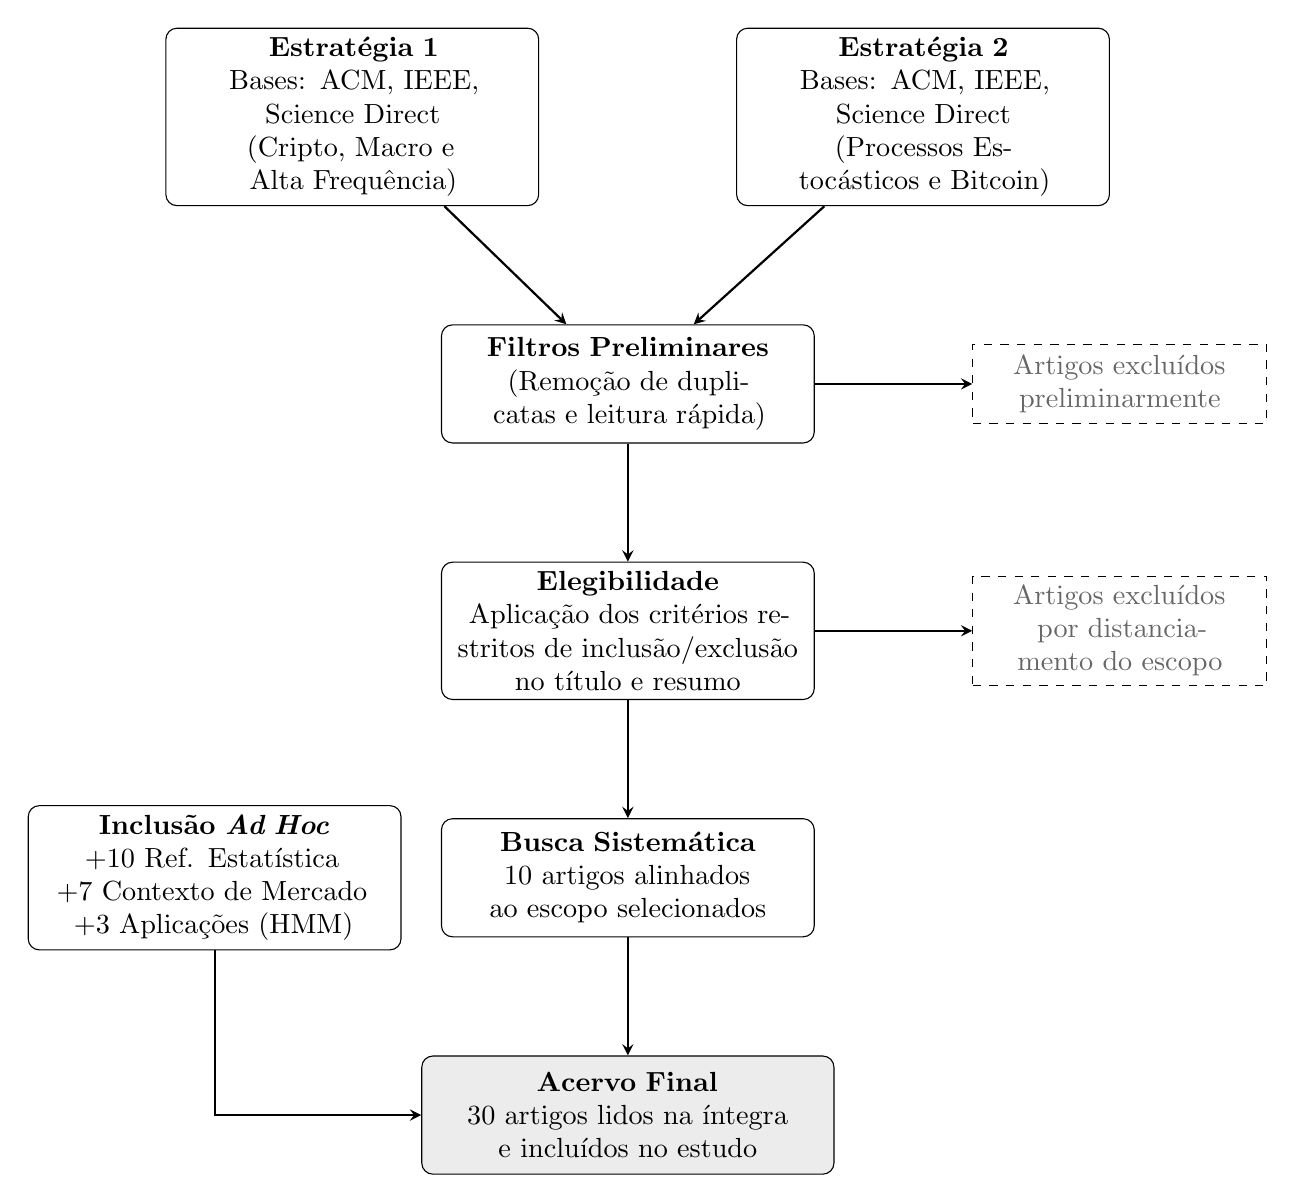
\begin{tikzpicture}[
        node distance=1.5cm and 2cm,
        box/.style={rectangle, draw, rounded corners, text width=4.5cm, align=center, minimum height=1.5cm},
        sidebox/.style={rectangle, draw, dashed, text width=3.5cm, align=center, minimum height=1cm, text=gray!80!black},
        arrow/.style={thick,->,>=stealth}
        ]

        \node (boxA) [box] {\textbf{Estratégia 1}\\Bases: ACM, IEEE, Science Direct\\(Cripto, Macro e Alta Frequência)};
        \node (boxB) [box, right=of boxA, xshift=0.5cm] {\textbf{Estratégia 2}\\Bases: ACM, IEEE, Science Direct\\(Processos Estocásticos e Bitcoin)};

        \node (boxC) [box, below=1.5cm of boxA, xshift=3.5cm] {\textbf{Filtros Preliminares}\\(Remoção de duplicatas e leitura rápida)};
        \node (exclC) [sidebox, right=of boxC] {Artigos excluídos preliminarmente};

        \node (boxD) [box, below=1.5cm of boxC] {\textbf{Elegibilidade}\\Aplicação dos critérios restritos de inclusão/exclusão no título e resumo};
        \node (exclD) [sidebox, right=of boxD] {Artigos excluídos por distanciamento do escopo};

        \node (boxE) [box, below=1.5cm of boxD] {\textbf{Busca Sistemática}\\10 artigos alinhados ao escopo selecionados};
        \node (boxF) [box, left=0.5cm of boxE] {\textbf{Inclusão \textit{Ad Hoc}}\\+10 Ref. Estatística\\+7 Contexto de Mercado\\+3 Aplicações (HMM)};

        \node (boxG) [box, below=1.5cm of boxE, fill=gray!15, text width=5cm] {\textbf{Acervo Final}\\30 artigos lidos na íntegra e incluídos no estudo};

        \draw [arrow] (boxA) -- (boxC);
        \draw [arrow] (boxB) -- (boxC);
        \draw [arrow] (boxC) -- (exclC);
        \draw [arrow] (boxC) -- (boxD);
        \draw [arrow] (boxD) -- (exclD);
        \draw [arrow] (boxD) -- (boxE);
        \draw [arrow] (boxE) -- (boxG);
        \draw [arrow] (boxF) |- (boxG);

    \end{tikzpicture}
    \fonte{Elaborado pelos autores (2026).}
\end{figure}

% ---------------------------------------------------------------
\section{Referencial teórico}
\label{sec:referencial}

Esta seção aborda a definição de moedas virtuais, com foco específico nas criptomoedas.
Em seguida, são apresentados os fundamentos analíticos do estudo, explicando o comporta-
mento das séries temporais financeiras, as Cadeias de Markov e suas aplicações, bem como
os Modelos Ocultos de Markov, do inglês \textit{Hidden Markov Model} (HMM). Por fim, detalha-se o processo de discretização de
dados, seguido pela apresentação e justificativa das métricas de avaliação utilizadas.

\subsection{Mercado financeiro e ativos digitais}

\subsubsection{Moedas virtuais}

Moedas virtuais são descritas de acordo com \citeonline{CHUEN} como sendo uma das
formas alternativas ao sistema clássico de moedas fiduciárias já estabelecido. De acordo
com a definição apresentada por \citeonline{fatf2014virtual}, uma moeda virtual é
uma representação digital de valor que pode ser negociada digitalmente e exercer funções
semelhantes às da moeda, como meio de troca, unidade de conta e reserva de valor, embora,
na definição original, não possua curso legal. Um dos meios de pagamentos virtuais mais
conhecidos é o Bitcoin, que é, na verdade, uma criptomoeda como apontado por \citeonline{CHUEN}.

\subsubsection{Criptomoedas}

Criptomoedas são definidas como ``moedas digitais conversíveis'' e em outras legislações
como ``equivalente digital a dinheiro'' \cite{papadopoulos2024blockchain}. De todo modo, essas
definições são aplicadas às criptomoedas que são convertidas para moedas oficiais utilizando
mercados digitais e sites de câmbio. De todo modo, moedas digitais não podem ser
consideradas dinheiro sob o olhar clássico \cite{papadopoulos2024blockchain}.

\subsubsection{Bitcoin}

Bitcoin foi a primeira criptomoeda de código aberto descentralizada criada, e é uma das
formas mais populares para pagamentos digitais \cite{CHUEN}.
O Bitcoin é tido como modelo e fonte de código para criptomoedas emergentes, embora nem
todas sigam seu modelo, como visto por \citeonline{papadopoulos2024blockchain}. O Bitcoin nasce com
o trabalho de \citeonline{nakamoto2008bitcoin} com o objetivo de ser uma alternativa aos pagamentos
baseados em fidúcia, criando um sistema \textit{peer-to-peer} (ponto a ponto) baseado em provas
criptográficas (usando de chaves públicas e privadas), assim permitindo que duas partes
efetuem pagamentos sem a necessidade de uma terceira entidade de confiança, formando
assim o ponto a ponto. Em seu trabalho \citeonline{nakamoto2008bitcoin} propõe que nós da rede atuem
como validadores das transações realizadas dentro do sistema.
As transações são definidas como um encadeamento de assinaturas digitais, como
podemos observar na \autoref{fig:bitcoin_transacao}. Para realizar uma transferência o proprietário remetente
transfere o valor assinando o \textit{hash} da transação anterior e a chave pública do proprietário
destinatário, adicionando ambos ao final da transação.

\begin{figure}[htbp]
    \centering
    \caption{Transações no modelo Bitcoin.}
    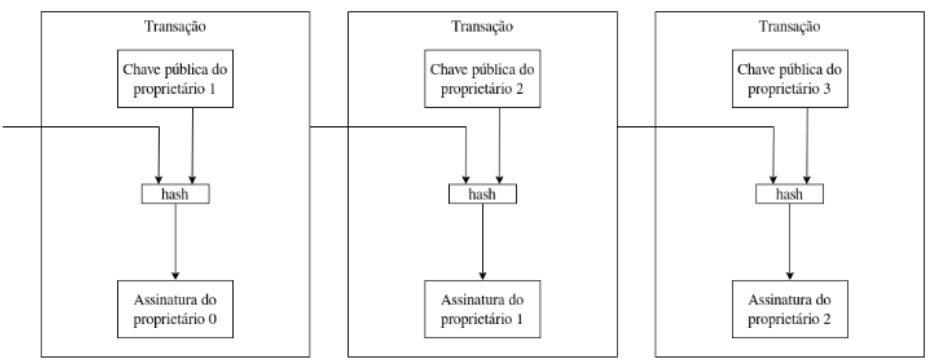
\includegraphics[width=0.8\textwidth]{images/Bitcoin.png}
    \fonte{\cite{nakamoto2008bitcoin}, adaptado pelos autores.}
    \label{fig:bitcoin_transacao}
\end{figure}

Em seu trabalho \citeonline{nakamoto2008bitcoin} descreve que as transações realizadas no sistema são publicamente anunciadas e a validade das
transações se baseia em um mecanismo de consenso baseado em poder computacional
(Proof-of-Work). Se a maioria do poder computacional da rede validar um bloco de
transações, então este bloco é adicionado ao histórico da rede através de um sistema
de validação temporal (timestamp) diferente de outros sistemas que dependem de uma
entidade central administradora, cada bloco possui informações sobre os blocos anteriores
fazendo assim um encadeamento dos blocos (blockchain). Contudo o sistema precisa de
um meio de validar se um proprietário não realizou uma transação dupla, gastando uma
mesma moeda duas vezes, e para isso o sistema conta com um serviço chamado timestamp.

\subsubsection{Timestamp}

Para \citeonline{nakamoto2008bitcoin}, o \textit{timestamp} não é apenas ``data e hora'', mas sim um sistema
de validação temporal descentralizado. Esse sistema é responsável por aplicar
a função \textit{hash} em blocos de transações, \textit{hash} é uma função matemática criptográfica que transforma qualquer conjunto de dados em uma sequência única de caracteres de tamanho
fixo, sendo único para cada bloco. O serviço depois é responsável por divulgar o \textit{hash} do
bloco pela rede. Cada novo bloco emitido pelo sistema inclui o \textit{hash} do bloco anterior em
sua composição, formando assim uma cadeia (\textit{chain}) onde cada bloco subsequente reafirma
a validade dos blocos anteriores. Podemos observar esse funcionamento na \autoref{fig:bitcoin_transacao2}, onde o
serviço de \textit{timestamp} aplica a função a um bloco, depois o hash é propagado e usado
para compor a função \textit{hash} do próximo bloco.

\begin{figure}[htbp]
    \centering
    \caption{Funcionamento do serviço de timestamp.}
    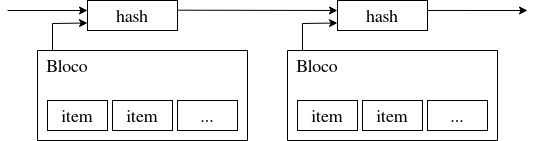
\includegraphics[width=0.8\textwidth]{images/Timestamp.png}
    \fonte{\cite{nakamoto2008bitcoin}, adaptado pelos autores.}
    \label{fig:bitcoin_transacao2}
\end{figure}

\subsubsection{Proof-of-Work}
Para implementar um serviço timestamp como descrito anteriormente, é utilizado outro sistema, o \textit{Proof-of-Work} (Prova de trabalho). As provas de trabalho envolvem aplicar uma
função hash a um bloco e verificar se esse hash começa com uma quantidade específica de zeros. Para chegar em um hash que respeite essa condição é adicionado
ao bloco um número que é utilizado apenas uma vez (Nonce) e depois a função hash é aplicada ao bloco, uma vez que o hash não respeite a regra basta escolher outro 
nonce e aplicar a função hash novamente até que o hash respeite a regra imposta \cite{nakamoto2008bitcoin}. 

Essa prova de trabalho é essencialmente um modelo de um voto por CPU. O incentivo para que os nós participem da prova de trabalho é que os participantes são recompensados,
o primeiro nó a conseguir achar o hash para o bloco receberá moedas criadas recentemente \cite{CHUEN}.

Podemos observar na \autoref{fig:blockchain} o funcionamento do encadeamento dos blocos.

\begin{figure}[H]
    \centering
    \caption{Encadeamento de blocos na blockchain.}
    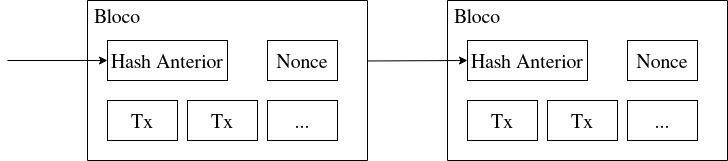
\includegraphics[width=0.85\textwidth]{images/Blockchain}
    \fonte{\cite{nakamoto2008bitcoin}, adaptado pelos autores.}
    \label{fig:blockchain}
\end{figure}

\subsubsection{Rede}
Os passos de funcionamento da rede são:

\begin{enumerate}
    \item Novas transações são transmitidas a todos os nós.
    \item Cada nó coleta as novas transações e gera um bloco.
    \item Cada nó tenta encontrar a prova de dificuldade para seu bloco.
    \item Quando um nó encontra a prova de dificuldade ele transmite a prova para toda a rede.
    \item Os nós da rede aceitam o bloco transmitido apenas se todas as transações são válidas e não foram gastas anteriormente.
    \item Os nós expressam o consenso de aprovação para o bloco usando o hash do bloco aceito para criar o próximo bloco da cadeia.
\end{enumerate}

\subsection{Macroeconomia e Bitcoin}
Conforme demonstrado por \citeonline{BENOMRANE2025}, análises baseadas em retornos diários mostram-se inadequadas para a avaliação de eventos macroeconômicos em 
criptoativos. Uma vez que os choques gerados por indicadores de inflação são incorporados nos preços de forma quase instantânea, o recurso a uma frequência diária 
resultaria no mascaramento dessas reações intradiárias. Portanto, para analisar melhor a volatilidade do Bitcoin, serão usadas janelas de fechamento de 5 minutos,
como demonstrado por \citeonline{GONZALEZ2025}, o intervalo de 5 minutos possui os resultados mais acurados, intervalos de granularidade mais fina possuem muito ruído o que pode gerar
distorção na volatilidade e nos resultados do estudo.

\subsection{Séries temporais financeiras}

Uma série temporal é qualquer conjunto de observações ordenadas no tempo \cite{morettin2018analise}. Frequentemente, uma série temporal discreta é obtida pela amostragem de uma série contínua em intervalos de tempo iguais. É importante notar que aquilo que se denomina série temporal corresponde, na realidade, a apenas uma das muitas trajetórias possíveis que poderiam ter sido observadas a partir de um determinado processo, fenômeno ou evento \cite{morettin2018analise}. A série de retornos do Bitcoin configura uma série univariável e unidimensional, isto é, dado o parâmetro tempo $t$, obtém-se o retorno do ativo no instante correspondente, e sua série descrita sob intervalos de tempo constante configura uma série temporal discreta.

Segundo \citeonline{morettin2018analise}, a análise de séries temporais pode ser utilizada para alcançar diferentes objetivos, entre os quais se destacam

\begin{itemize}
    \item investigar o mecanismo gerador da série, isto é, compreender o que origina o dado observado
    \item realizar previsões de valores futuros, sejam elas de curto ou de longo prazo
    \item descrever e analisar o comportamento da série, identificando a existência de tendências, ciclos e variações sazonais
    \item buscar periodicidades relevantes nos dados.
\end{itemize}

Dentre esses objetivos, este trabalho se concentra na previsão de valores futuros. Para isso, é necessário antes compreender 
o comportamento da série de retornos do Bitcoin e as propriedades que a distinguem de outras séries temporais, apresentadas a seguir.

\subsubsection{Propriedades de séries temporais financeiras}

As séries financeiras, embora compartilhem da estrutura geral descrita acima, possuem propriedades particulares que as distinguem de outras séries temporais. Em geral, não se trabalha com a série de preços, mas com a série de retornos, por razões tanto estatísticas quanto econômicas. Uma das transformações mais empregadas é o retorno logarítmico, também denominado retorno composto contínuo, definido como

\begin{equation}
    r_t = \log\!\left(\frac{P_t}{P_{t-1}}\right) = p_t - p_{t-1} = \Delta \log(P_t),
    \label{retorno_logaritmico}
\end{equation}

em que $P_t$ é o preço do ativo no instante $t$ e $p_t = \ln(P_t)$ denota o logaritmo natural do preço nesse mesmo 
instante \cite{morettin2018analise}. A passagem para os retornos logarítmicos confere à série propriedades 
convenientes para a modelagem, tais como a aditividade temporal e a estabilização da variância. Por exemplo, se o 
preço de um ativo cai de 100 para 80 e depois volta a 100, os retornos simples são de $-20\%$ e $+25\%$, cuja soma não é zero. 
Já os retornos logarítmicos são $\ln(0{,}8) \approx -0{,}223$ e $\ln(1{,}25) \approx +0{,}223$, que se anulam. 
De modo geral, o retorno logarítmico acumulado em vários períodos é a soma dos retornos logarítmicos de cada período.

\subsubsection{Estacionariedade e autocorrelação}
\label{subsubsec:estacionariedade}

Uma das suposições mais recorrentes na análise de séries temporais é a de estacionariedade, segundo a qual a série se desenvolve aleatoriamente no tempo em torno de uma média constante, refletindo um comportamento de equilíbrio e constância. Na prática, as séries temporais não costumam apresentar algum tipo de estacionariedade no seu comportamento. As séries financeiras, em particular, costumam exibir tendências, fases de alta, de baixa e de lateralização, o que afasta a propriedade de estacionariedade quando se trabalha diretamente com a série de preços \cite{morettin2018analise}.

É justamente esse comportamento que motiva a transformação dos preços em retornos, ao utilizar a diferença de logaritmos se busca uma série mais próxima da estacionariedade, condição que é necessária para grande parte das técnicas de modelagem de sistemas de previsão. Em relação à autocorrelação, os retornos financeiros apresentam um padrão peculiar, sendo, em geral, não autocorrelacionados de maneira linear \cite{morettin2018analise}, o que na prática significa que os retornos passados não servem para realizar as previsões na série de maneira linear.

\subsubsection{Fatos estilizados dos Retornos financeiros}

Os retornos financeiros apresentam características peculiares que não se observam em outras séries temporais. Tipicamente, eles não exibem tendências nem sazonalidade. Os principais fatos estilizados podem ser resumidos nos seguintes pontos \cite{morettin2018analise}:
\begin{enumerate}
    \item os retornos são, em geral, não autocorrelacionados de maneira linear;
    \item as séries de retornos apresentam agrupamentos de volatilidade ao longo do tempo, de modo que períodos de alta variabilidade tendem a ser seguidos por períodos igualmente voláteis, e vice-versa;
    \item a distribuição dos retornos apresenta caudas mais pesadas do que a distribuição normal e, embora aproximadamente simétrica, é em geral leptocúrtica;
\end{enumerate}

\subsection{Processos estocásticos e Cadeias de Markov}
\label{sec:processos_estocasticos}

Esta seção destina-se a apresentar parte da fundamentação teórica que dará suporte ao desenvolvimento da pesquisa. O texto introduz a noção geral de processos 
estocásticos e afunila para a apresentação das Cadeias de Markov, modelo este que será adotado nas etapas seguintes do trabalho, compreendendo suas propriedades e 
aplicações práticas.

\subsubsection{Eventos elementares e Aleatórios}
O conceito de evento elementar é a noção primitiva na formulação axiomática da teoria das probabilidades. Para cada problema investigado, deve-se definir 
previamente o que constitui o resultado mais básico e indivisível do experimento, formando assim o universo de possibilidades, que é denominado conjunto de 
eventos elementares e denotado por $E$ \cite{FISZ}.

Para ilustrar, \citeonline{FISZ} fornece o exemplo do lançamento de um dado de seis faces. Pode-se denotar a ocorrência de uma face específica i 
(onde $1 \leq i \leq 6$) com a notação $e_i$. Nesse cenário, cada resultado individual do dado é um evento elementar, tal que $e_i \in E$.

A partir da estrutura de $E$, estabelece-se um conjunto $Z$ formado por subconjuntos de eventos elementares de $E$. Esse conjunto $Z$ é denominado campo de Borel, 
e os elementos que o compõem são chamados de eventos aleatórios desde que a estrutura de $Z$ atenda às seguintes propriedades \cite{FISZ}:

\begin{enumerate}
    \item O campo $Z$ possui como um de seus elementos o próprio conjunto $E$ em sua totalidade (caracterizando o evento certo).
    \item O campo $Z$ possui como um de seus elementos o conjunto vazio $\emptyset$ (caracterizando o evento impossível).
    \item Se um número finito ou enumerável de eventos $A_1, A_2, \dots A_n \in Z$, então a sua união (ou alternativa) também pertence a $Z$.
    \item Se os eventos $A_1$ e $A_2$ pertencem a $Z$, então a sua diferença ($A_1 - A_2$) também pertence a $Z$.
    \item Se um número finito ou enumerável de eventos $A_1, A_2, \dots A_n \in Z$, então o seu produto (ou interseção) também pertence a $Z$.
\end{enumerate}

Como observado por \citeonline{FISZ} a conjugação das propriedades 1 e 4 gera uma consequência: evento complementar. Como o conjunto universo $E$ pertence a $Z$ (Propriedade 1) 
e o campo é fechado para a diferença entre dois de seus elementos (Propriedade 4), então nota-se que a diferença $E - A$ também pertence a $Z$. Dessa forma, garante-se que, 
se um determinado evento pertence ao campo de Borel, o seu exato oposto (o seu complemento) também será, obrigatoriamente, um evento aleatório.

\subsection{Variáveis Aleatórias}

Seja $E$ o conjunto de eventos elementares e $e \in E$ um evento elementar. Definimos $X(e)$ como uma função real de valor único sobre o conjunto $E$, isto é, $X: E \to 
\mathbb{R}$. Para um dado subconjunto $S \subseteq \mathbb{R}$, denotamos por $A$ a imagem inversa de $S$.
Uma função $X$ definida no conjunto $E$ é chamada de variável aleatória se a imagem inversa de qualquer intervalo $I$ no eixo real for um evento aleatório.
Definimos que a probabilidade de a variável aleatória $X$ assumir um valor dentro do intervalo $I$ é igual à probabilidade de sua imagem inversa $A$, ou seja:

\begin{equation}
    P(X \in I) = P(A)
\end{equation} \cite{FISZ}

Um exemplo mais prático de variáveis aleatórias é demonstrado por \citeonline{ROSS}, no qual se soma o resultado do lançamento de dois dados:

\begin{align*}
    P(X = 2)  &= P(\{(1,1)\}) = \frac{1}{36} \\
    P(X = 3)  &= P(\{(1,2), (2,1)\}) = \frac{2}{36} \\
    P(X = 4)  &= P(\{(1,3), (2,2), (3,1)\}) = \frac{3}{36} \\
    P(X = 5)  &= P(\{(1,4), (2,3), (3,2), (4,1)\}) = \frac{4}{36} \\
    P(X = 6)  &= P(\{(1,5), (2,4), (3,3), (4,2), (5,1)\}) = \frac{5}{36} \\
    P(X = 7)  &= P(\{(1,6), (2,5), (3,4), (4,3), (5,2), (6,1)\}) = \frac{6}{36} \\
    P(X = 8)  &= P(\{(2,6), (3,5), (4,4), (5,3), (6,2)\}) = \frac{5}{36} \\
    P(X = 9)  &= P(\{(3,6), (4,5), (5,4), (6,3)\}) = \frac{4}{36} \\
    P(X = 10) &= P(\{(4,6), (5,5), (6,4)\}) = \frac{3}{36} \\
    P(X = 11) &= P(\{(5,6), (6,5)\}) = \frac{2}{36} \\
    P(X = 12) &= P(\{(6,6)\}) = \frac{1}{36}
\end{align*}

Neste caso $X$ pode assumir um número contável de valores $(2 \leq X \leq 12)$, então $X$ é uma variável aleatória discreta.

\subsubsection{Processos estocásticos}
Conforme definido por \citeonline{FISZ} e \citeonline{ROSS}, um processo estocástico é uma coleção de variáveis aleatórias parametrizadas por $t$, comumente denotada 
por $\{X_t, t \in T\}$. O conjunto $T$ é chamado de conjunto de índices do processo e é interpretado como o tempo. Sendo assim, $X_t$ representa o estado em que o 
processo se encontra no exato instante $t$. A classificação estrutural de um processo estocástico depende diretamente da natureza do seu conjunto de índices $T$. Quando 
$T$ é um conjunto enumerável, o modelo é categorizado como um processo de tempo discreto. Por outro lado, se $T$ for um intervalo contínuo na reta dos números reais, o 
processo é classificado como de tempo contínuo. Por fim, o conjunto que engloba todos os valores possíveis que $X_t$ pode assumir ao longo da evolução do sistema é 
denominado \textit{espaço de estados} do processo \cite{ROSS}.

\subsubsection{Cadeias de Markov}
Conforme \citeonline{ROSS}, seja $\{X_n, n = 0, 1, 2, \dots\}$ um processo estocástico em que $X_n$ assume valores em um espaço de estados composto por inteiros não negativos. Quando $X_n = i$, 
diz-se que o processo se encontra no estado $i$ no instante $n$. Supõe-se que, sempre que o processo está no estado $i$, existe uma probabilidade fixa $P_{ij}$ de que 
o próximo estado seja $j$. Matematicamente, essa condição é expressa por:

\begin{equation}
    P(X_{n+1} = j \mid X_n = i, X_{n-1} = i_{n-1}, \dots, X_1 = i_1, X_0 = i_0) = P_{ij}
\end{equation}

Um processo estocástico que satisfaz a equação para todos os estados $i_0, i_1, \dots, i_{n-1}, i, j$ e para todo instante $n \geq 0$ é denominado Cadeia de Markov \cite{ROSS}. 
Em outras palavras, o estado futuro $X_{n+1}$ é condicionalmente independente de todo o histórico passado do processo, dependendo exclusivamente do estado presente 
$X_n$.

As probabilidades de transição $P_{ij}$ podem ser organizadas em uma matriz $\mathbf{P}$ \cite{ROSS}, estruturada da seguinte forma:

\begin{equation*}
\mathbf{P} = \begin{pmatrix}
    P_{00} & P_{01} & P_{02} & \cdots \\
    P_{10} & P_{11} & P_{12} & \cdots \\
    \vdots & \vdots & \vdots & \ddots \\
    P_{i0} & P_{i1} & P_{i2} & \cdots \\
    \vdots & \vdots & \vdots & \ddots
\end{pmatrix}
\end{equation*}

\vspace{0.5cm}

Como essas probabilidades representam a chance de transição de um estado para outro, e considerando que o processo obrigatoriamente fará uma transição para algum 
estado (incluindo a possibilidade de permanecer no mesmo estado atual), os elementos da matriz devem satisfazer as seguintes condições:

\begin{equation*}
    P_{ij} \geq 0, \quad i,j \geq 0; \qquad \sum_{j=0}^{\infty} P_{ij} = 1, \quad i = 0, 1, \dots
\end{equation*}

\subsection{Cadeias de Markov de alta Ordem}
Em seu estudo \cite{URQUHART} conclui que os retornos do Bitcoin possuem indícios de comportamento aleatório, porém na literatura mais recente \cite{NASCIMENTO} não só revela 
evidências de que a série do Bitcoin possui memória como determinam a magnitude dessa memória usando modelos estatísticos. Um modelo de cadeias de Markov de Alta ordem é 
apresentado por \citeonline{RAFTERY1985} como uma alternativa aos modelos convencionais que possuem o número de parâmetros independentes descritos por:

$m^l(m - 1)$, onde $m$ é o número de estados e $l$ a ordem da cadeia de markov, o modelo introduzido por \citeonline{RAFTERY1985} foi posteriormente chamado de Mistura de 
Distribuições de Transição, do inglês \textit{Mixture Transition Distribution} (MTD), e utiliza de $m(m -1) + (l - 1)$ parâmetros independentes e é descrito por:

\begin{equation}
    P[X_{t}=j_{0} \mid X_{t-1}=j_{1}, \dots, X_{t-l}=j_{l}] = \sum_{i=1}^{l}\lambda_{i}q_{j_{0}j_{i}}
\end{equation}

onde a probabilidade condicional de observar o estado $j_0$ no instante $t$ é expressa como uma combinação linear das contribuições individuais de cada um dos estados 
passados ($X_{t-1}, X_{t-2}, \dots, X_{t-l}$).

Alternativamente, o modelo pode ser representado em sua forma matricial. Para tanto, define-se o vetor coluna $X_t = (X_t(1), \dots, X_t(m))^\prime$, onde $X_t(j) = 1$ 
se o processo estiver no estado $j$ no instante $t$, e $0$ caso contrário. Analogamente, seja $\hat{X}_t = (\hat{X}_t(1), \dots, \hat{X}_t(m))^\prime$ o vetor cujos 
elementos $\hat{X}_t(j)$ representam a probabilidade condicional $P[X_t = j \mid X_{t-1} = j_1, X_{t-2} = j_2, \dots]$. Desse modo, a formulação linear pode ser 
reescrita como:

\begin{equation}
    \hat{X}_t = \sum_{i = 1}^{l} \lambda_i Q X_{t-i}
\end{equation}

Note que, quando $l = 1$, a equação reduz-se a uma cadeia de Markov de primeira ordem clássica com matriz de transição $Q$. No entanto, adota-se aqui a convenção de 
\citeonline{RAFTERY1985}, na qual a soma dos elementos de cada coluna de $Q$ é igual a 1, diferindo do enfoque tradicional estruturado por linhas.

Para chegar nos melhores pesos para cada $t$ \citeonline{RAFTERY1985} utiliza do Critério de Informação Bayesiano, do inglês \textit{Bayesian Information Criterion} 
(BIC), com o objetivo de minimizar esse critério. O BIC é definido como:

\begin{equation}
    BIC = -2LL + p \times log(n)    
\end{equation}

onde $LL$ é o logaritmo da função de verossimilhança do modelo, $p$ é o número de parâmetros independentes e $n$ é o número de componentes da função logaritmo de 
verossimilhança \cite{RAFTERY1985}

\subsection{Modelos Ocultos de Markov (HMM)}

Segundo \citeonline{Ghahramani}, o HMM é uma ferramenta utilizada para representar
distribuições de probabilidades sobre uma sequência de observações dentro de uma série temporal. 
O objeto observado pode ser um símbolo de um alfabeto discreto, um valor real, um número inteiro ou qualquer 
outro objeto sobre o qual se possa definir uma distribuição de probabilidade.

Um HMM consiste em dois processos estocásticos: o primeiro é a Cadeia de Markov, caracterizada por estados e 
probabilidades de transição, onde esses estados não são visíveis externamente (ou seja, são ocultos) e o segundo é um 
processo estocástico que produz emissões observáveis atreladas a cada um dos estados \cite{Dymarski}.

Os HMMs são comumente utilizados para a análise e observação de séries temporais em diferentes contextos. São aplicados na área de biologia molecular para a 
identificação de genes \cite{MA2026101729}, reconhecimento de fala para a modelagem de fonemas \cite{jm3}, dentre outras áreas \cite{Dymarski}. Neste trabalho, 
utilizaremos um modelo HMM aplicado ao setor financeiro, mais especificamente voltado aos ativos digitais (Bitcoin).

Para compreender a aplicação prática do HMM, é necessário detalhar a relação entre os dados visíveis (emissões observáveis)
e os estados ocultos que o sistema infere de maneira indireta.
\subsubsection{Estados Ocultos e Observáveis}

Em um HMM, o modelo é categorizado em dois conjuntos fundamentais,
os estados ocultos e as observações (ou estados observáveis). Os estados observáveis correspondem aos dados empíricos extraídos de maneira 
direta da série temporal, refletindo as medições quantificáveis da realidade. Em contrapartida, os estados ocultos representam a dinâmica 
interna e estocástica do sistema. Embora sejam invisíveis ao observador externo, esses estados ocultos governam o comportamento do 
modelo e influenciam diretamente a distribuição de probabilidade responsável por gerar as emissões observáveis a cada instante \cite{Dymarski}. 
No contexto desta pesquisa, essas emissões observáveis correspondem aos dados empíricos extraídos diretamente da série temporal, refletindo os retornos quantificáveis 
do ativo.

\begin{figure}[htbp]
    \centering
    \caption{Modelo ilustrativo para a generalização dos estados.}
    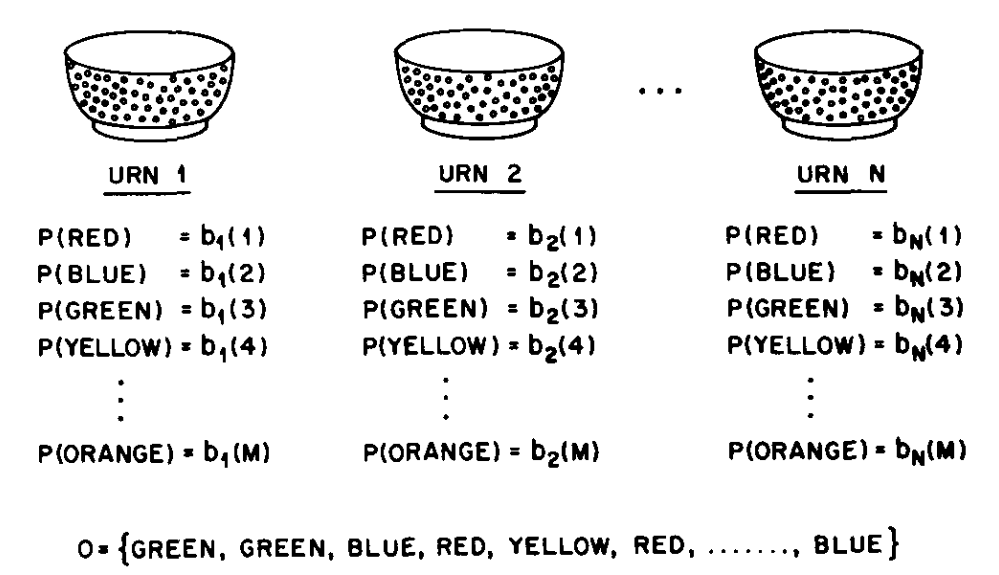
\includegraphics[width=0.8\textwidth]{HMM_Urna.png}
    \fonte{\cite{Rabiner1989}}
    \label{fig:hmm_exemplo}
\end{figure}

Podemos entender melhor a dinâmica entre os diferentes estados através do exemplo ilustrado na \autoref{fig:hmm_exemplo}.
Suponhamos que temos uma sequência observada de bolas coloridas que são sorteadas em diferentes momentos. 
Nossos estados observáveis são as cores das bolas que conseguimos ver sair, no exemplo ilustrado, 
verde (\textit{GREEN}), azul (\textit{BLUE}), vermelho (\textit{RED}) e amarelo (\textit{YELLOW}), formando a sequência 
de observações $O$.

Nós sabemos que a cor da bola sorteada é influenciada de maneira indireta pela urna da qual ela foi retirada (Urna 1, Urna 2, \dots, Urna $N$). Como a urna escolhida a 
cada passo não é registrada diretamente na nossa sequência de observações (nós enxergamos apenas as cores das bolas sorteadas), essas urnas representam os estados 
ocultos do nosso sistema, sendo as responsáveis por emitir as probabilidades de observarmos cada cor (representadas pelas funções de emissão $P(COR) = b_n(m)$).

Compreendida a dinâmica intuitiva dos estados, a próxima etapa consiste em formalizar os componentes principais que
definem um HMM.

\subsubsection{Componentes do modelo HMM}

O HMM possui características herdadas de outros processos estocásticos, como a Cadeia de Markov.
Formalmente, conforme definido por \citeonline{Kuinchtner2018}, o HMM é caracterizado pelos seguintes componentes:

\begin{itemize}
    \item $N$, que representa o número de estados ocultos no modelo;
    
    \item $M = \{m_1, m_2, \dots, m_n\}$, que representa o conjunto de observações possíveis (símbolos observáveis), 
    onde estes dependem dos estados. Cada observação possui uma probabilidade distinta associada a cada estado;

    \item Uma matriz de transição de 
    estados $A = \{a_{ij}\}$, onde $a_{ij} = P(q_{t+1} = S_j \mid q_t = S_i) \ \forall \ i,j = 1, 2, \dots, N$, 
    exemplificada na Equação \ref{a_matriz}:

    \begin{equation}
        A = \begin{pmatrix}
            a_{i \to i} & a_{i \to j} \\
            a_{j \to i} & a_{j \to j}
        \end{pmatrix}
        \label{a_matriz}
    \end{equation}

    \item Uma matriz de probabilidade de emissão $B$, que representa a distribuição probabilística da emissão de um estado, 
    exemplificada na Equação \ref{b_matriz}, sendo esta a matriz que interliga os estados ocultos aos estados observáveis:

    \begin{equation}
        B = \begin{pmatrix}
            b_i(m_1) & b_i(m_2) & b_i(m_3) \\
            b_j(m_1) & b_j(m_2) & b_j(m_3)
        \end{pmatrix}
        \label{b_matriz}
    \end{equation}

    \item Um vetor $\pi$, que representa a distribuição de probabilidade inicial para cada um dos estados do sistema, 
    exemplificado na Equação \ref{pi_matriz}:

    \begin{equation}
        \pi = \begin{pmatrix}
            \pi_i \\
            \pi_j
        \end{pmatrix}
        \label{pi_matriz}
    \end{equation}

    \item $\lambda$, que representa o próprio modelo de forma compactada, comumente denotado por $\lambda = (A, B, \pi)$.
\end{itemize}

A simples definição desses componentes não é suficiente para a análise preditiva, é preciso que o modelo seja capaz de interagir 
com os dados reais. Isso nos leva aos três desafios operacionais que permitem ao HMM realizar inferências e aprendizado.

\subsubsection{Avaliação, Decodificação e Aprendizado}

Segundo \citeonline{Rabiner1989}, para que os HMMs sejam úteis em aplicações reais, é necessário
solucionar três problemas fundamentais, que se apresentam da seguinte forma:

\begin{itemize}
    \item \textbf{Problema 1 (Avaliação):} Dada uma sequência de observações $O={O_1 O_2 \dots O_t}$ e um 
    modelo $\lambda = (A, B, \pi)$, como calculamos eficientemente $P(O|\lambda)$, isto é, a probabilidade
    de ocorrência da sequência de observações dado o modelo? \cite{Rabiner1989}

    O primeiro problema apresenta-se como um problema de avaliação, no qual, dada uma sequência de observações, como
    calcular a probabilidade de ela ter sido produzida pelo modelo? Esse problema também pode ser analisado pela 
    perspectiva de seleção de modelos, em que se avaliam diferentes modelos com o objetivo de 
    identificar qual obtém a maior probabilidade de ter gerado as observações fornecidas.


    \item \textbf{Problema 2 (Decodificação):} Dada a sequência de observações $O={O_1 O_2 \dots O_t}$, e o modelo $\lambda = (A, B, \pi)$, 
    como escolhemos uma sequência de estados correspondente $Q={q_1 q_2 \dots q_t}$ que seja ótima? Ou seja, que maximize a probabilidade
    da ocorrência da sequência observada. \cite{Rabiner1989}

    O segundo problema representa aquilo que buscamos de fato ao utilizar um modelo treinado HMM. Fundamentalmente, 
    o objetivo em um HMM é descobrir qual é a sequência de estados ocultos que melhor explica (maximiza a probabilidade de) termos 
    obtido a sequência observada $O$.

    \item \textbf{Problema 3 (Aprendizado):} Como ajustamos os parâmetros do modelo $\lambda = (A, B, \pi)$ para maximizar $P(O|\lambda)$? \cite{Rabiner1989}
    
    O Problema 3 refere-se ao treinamento do HMM, no qual buscamos otimizar os parâmetros do modelo $\lambda = (A, B, \pi)$ 
    para descrever da melhor forma possível como uma sequência de observações é gerada. Esse problema é fundamental pois nos permite 
    adaptar o modelo aos dados reais e, assim, otimizar suas predições.

\end{itemize}

As soluções para os problemas descritos são resolvidas através de algoritmos fundamentados em programação dinâmica,
como os algoritmos \textit{Forward}, \textit{Viterbi} e \textit{Baum-Welch}. O uso destes algoritmos torna o HMM 
uma solução computacionalmente viável, a subseção a seguir é dedicada às especificidades de cada um desses algoritmos e à sua 
utilidade na estrutura do modelo.

\subsubsection{Algoritmos clássicos}

\paragraph{Algoritmo \textit{Forward}}

O algoritmo \textit{Forward} é utilizado para a resolução do primeiro problema descrito na seção anterior (Avaliação). 
Ele utiliza programação dinâmica, empregando uma tabela para armazenar valores intermediários conforme constrói 
a probabilidade da sequência de observações. O algoritmo calcula a probabilidade de obtermos aquela observação 
somando, de maneira eficiente, as probabilidades de todos os caminhos de estados ocultos possíveis que 
poderiam gerar aquela sequência de estados observados \cite{jm3}.

\begin{figure}[htbp]
    \centering
    \caption{Representação do processo do algoritmo \textit{Forward} para uma sequência de três observações.}
    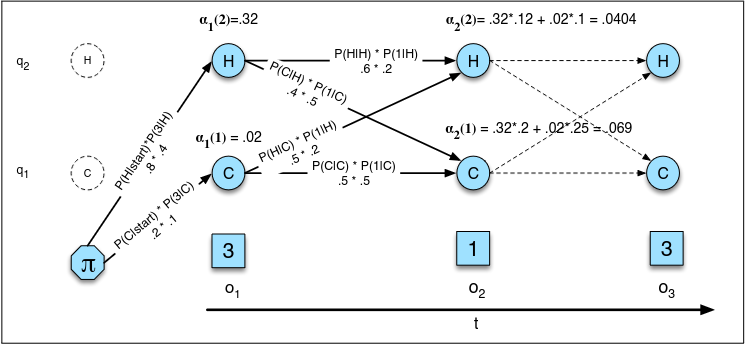
\includegraphics[width=0.8\textwidth]{Forward.png}
    \fonte{\cite{jm3}}
    \label{fig:diagrama_forward}
\end{figure}

Cada célula da \autoref{fig:diagrama_forward}, denotada por $\alpha_t(j)$, representa a probabilidade 
de estar num estado $j$ no instante $t$ dadas as observações anteriores. O valor de cada célula $\alpha_t(j)$ é 
calculado através da soma das probabilidades dos caminhos que levam até ela \cite{jm3}:

\begin{equation}
    \alpha_t(j) = P(o_1, o_2, \dots, o_t, q_t = j | \lambda)
    \label{probabilidade_celula}
\end{equation}

Onde $q_t$ representa o estado no instante $t$, sendo este um estado oculto do sistema, e $\lambda$ representa os 
parâmetros do modelo. O valor para a célula $\alpha_t(j)$ é dado pela soma das probabilidades de todos os caminhos 
que nos levam até à mesma; portanto, para um estado $j$, o valor de $\alpha_t(j)$ é calculado da seguinte forma \cite{jm3}:

\begin{equation}
    \alpha_t(j) = \sum_{i=1}^{N} \alpha_{t-1}(i) a_{ij} b_j(o_t)
    \label{probabilidade_de_alfa}
\end{equation}

Onde os fatores da multiplicação são:

\begin{itemize}
    \item $\alpha_{t-1}(i)$: Representa o valor de probabilidade \textit{forward} acumulado para o estado $i$ no instante de tempo anterior ($t-1$).
    \item $a_{ij}$: Representa a probabilidade de transição do estado $i$ para o estado $j$ (dada pela matriz de probabilidades de transição $A$ do modelo).
    \item $b_j(o_t)$: A probabilidade de emissão da observação $o_t$ dado o estado $j$.
\end{itemize}

\paragraph{Algoritmo de Viterbi}

O algoritmo de Viterbi é responsável por solucionar o problema de Decodificação de HMMs.
O algoritmo nos dá a sequência de estados ocultos que maximizam as probabilidades de termos uma sequência de observações $O$.

Tentar encontrar a melhor sequência calculando a probabilidade de todas as combinações possíveis de estados ocultos
(por exemplo, executando o algoritmo \textit{Forward} para cada combinação) exigiria um esforço computacional inviável, 
com um número exponencial de caminhos. Para contornar essa limitação, o algoritmo de Viterbi, de maneira similar 
ao \textit{Forward}, também é um algoritmo de programação dinâmica \cite{jm3}, porém, a
principal diferença reside no fato de que o algoritmo de Viterbi seleciona apenas o caminho de probabilidade 
máxima em cada etapa. Cada célula, denotada por $v_t(j)$, representa a probabilidade de o modelo estar no estado $j$ 
no instante $t$, tendo percorrido a sequência de estados mais provável até aquele momento \cite{jm3}, $v_t(j)$ é representado da
seguinte maneira:

\begin{equation}
    v_t(j) = \max_{q_1,\dots,q_{t-1}} P(q_1 \dots q_{t-1}, o_1, o_2 \dots o_t, q_t = j | \lambda)
    \label{probabilidade_viterbi}
\end{equation}

A probabilidade de Viterbi para um estado $j$ no instante atual $t$ é obtida extraindo a maior extensão possível dos caminhos anteriores: \cite{jm3}

\begin{equation}
    v_t(j) = \max_{i=1}^{N} v_{t-1}(i) a_{ij} b_j(o_t)
    \label{recursao_viterbi}
\end{equation}

Os três fatores responsáveis por estender o caminho e calcular a probabilidade na Equação \ref{recursao_viterbi} são:

\begin{itemize}
    \item $v_{t-1}(i)$: A probabilidade do caminho mais provável até o estado $i$ no instante de tempo anterior ($t-1$).
    \item $a_{ij}$: A probabilidade de transição do estado $i$ para o estado atual $j$ (obtida da matriz de transição $A$).
    \item $b_j(o_t)$: A probabilidade de emissão da observação $o_t$ dado que o modelo se encontra no estado $j$.
\end{itemize}

\paragraph{Algoritmo de Baum-Welch}

O algoritmo de Baum-Welch é utilizado para a resolução do problema de aprendizado inerente aos HMMs.
Este problema consiste em estimar os parâmetros do modelo $\lambda$, ou seja, as matrizes de transição dos estados ocultos ($A$) e das probabilidades
de emissão ($B$), dada uma sequência de observações $O$ e uma sequência de potenciais estados ocultos $Q$.

O método é um caso especial do algoritmo de Maximização da Expectativa (do inglês \textit{Expectation-Maximization} ou EM). Se trata de um algoritmo 
iterativo que calcula uma estimativa inicial para as probabilidades, em seguida, utiliza essas estimativas para derivar probabilidades cada vez 
melhores até que ocorra a convergência. 

Para um HMM real, não é possível calcular as contagens das transições e emissões diretamente de uma sequência de observações, pois os caminhos de estados percorridos 
pela máquina são ocultos. O algoritmo de Baum-Welch contorna essa limitação estimando essas contagens de forma iterativa. 
Ele faz isso calculando a probabilidade \textit{forward} para uma observação e, em seguida, dividindo essa probabilidade entre todos os diferentes 
caminhos que contribuíram para ela. Para que isso seja possível, além da probabilidade \textit{forward} ($\alpha$), o algoritmo 
requer a definição de uma probabilidade \textit{backward} ($\beta$) \cite{jm3}.

A probabilidade \textit{backward}, denotada por $\beta_t(i)$, é a probabilidade de observar a sequência do instante $t+1$ até o final ($T$), dado que o 
modelo está no estado $i$ no instante $t$ (e dado o modelo $\lambda$):

\begin{equation}
    \beta_t(i) = P(o_{t+1}, o_{t+2} \dots o_T \mid q_t = i, \lambda)
    \label{eq:probabilidade_backward}
\end{equation}

Assim como no algoritmo \textit{forward}, o cálculo da probabilidade \textit{backward} é realizado em três etapas:

\textbf{1. Inicialização:}
\begin{equation}
    \beta_T(i) = 1, \quad 1 \le i \le N
    \label{eq:inicializacao_backward}
\end{equation}

\textbf{2. Recursão:}
\begin{equation}
    \beta_t(i) = \sum_{j=1}^N a_{ij} b_j(o_{t+1}) \beta_{t+1}(j), \quad 1 \le i \le N, \ 1 \le t < T
    \label{eq:recursao_backward}
\end{equation}

\textbf{3. Término:}
\begin{equation}
    P(O \mid \lambda) = \sum_{j=1}^N \pi_j b_j(o_1) \beta_1(j)
    \label{eq:termino_backward}
\end{equation}

A partir da combinação das variáveis \textit{forward} ($\alpha$) e \textit{backward} ($\beta$), o algoritmo de Baum-Welch é capaz de calcular a 
probabilidade de estar em um estado específico em um dado momento, ajustando iterativamente os parâmetros do modelo para maximizar a probabilidade da 
sequência de observações fornecida no treinamento \cite{jm3}.

\subsubsection{Ótimos locais e reinícios}

\subsubsection{Escalonamento numérico}

\subsubsection{Previsão pelo filtro forward}

Dado o funcionamento e as características dos modelos preditivos que iremos utilizar para alcançar os objetivos do trabalho,
é de fundamental importância entender como iremos tratar os dados de retorno da série temporal do Bitcoin para a realização do treinamento
dos modelos. A próxima seção é dedicada a como iremos tratar e preparar os dados para estes modelos.

\subsection{Discretização e representação simbólica de séries temporais}

\subsubsection{Por que discretizar os retornos}

A discretização consiste no processo de projetar dados contínuos e sequenciais 
em um espaço simbólico finito, por meio de padrões probabilísticos concisos que 
comprimem a informação preservando seu conteúdo essencial \cite{Jha2021_arxiv}. No contexto 
deste trabalho, essa transformação é mais do que uma escolha metodológica, trata-se
de um requisito operacional, uma vez que as Cadeias de Markov são definidas sobre um espaço de estados discreto.
A análise da série de retornos do Bitcoin necessita que cada observação contínua seja 
mapeada em um símbolo pertencente a um alfabeto finito.

Além da exigência operacional imposta pelo modelo, há uma motivação empírica relevante para a discretização.
Conforme foi demonstrado por \citeonline{jjfinec}, o comportamento dos ativos do mercado de criptomoedas é fortemente
contaminado por ruídos de microestrutura e transações. Este ruído compromete a análise contínua dos retornos quando analisados
em janelas de alta frequência, podendo ser mitigado através de técnicas de discretização que eliminam pequenas flutuações causadas
por ruídos.

\subsubsection{Estratégia de discretização dos dados}
\label{discretizacao}

De maneira similar a \citeonline{ARAUJO}, a discretização é aplicada sobre os retornos logarítmicos da série 
(Equação~\ref{retorno_logaritmico}) e classifica cada retorno conforme o seu afastamento da média, medido em 
frações do desvio padrão. Dados uma média amostral $\overline{r}$ e um desvio padrão amostral $s$, 
estimados sobre um conjunto de retornos de referência, e um parâmetro $k > 0$, cada retorno $r(t)$ é mapeado 
em um símbolo segundo a relação

\begin{equation}
    \begin{aligned}
        \left( r(t) - \overline{r} \right) < -\frac{s}{k} &\iff -1 \\
        -\frac{s}{k} \leq \left( r(t) - \overline{r} \right) \leq \frac{s}{k} &\iff 0 \\
        \left( r(t) - \overline{r} \right) > \frac{s}{k} &\iff 1
    \end{aligned}
    \label{discretizacao_eq}
\end{equation}

em que os símbolos $-1$, $0$ e $1$ representam, respectivamente, uma queda significativa, uma oscilação pouco expressiva em 
torno da média e uma alta significativa. O parâmetro $k$ controla a largura da faixa central: quanto maior o valor de $k$, 
mais estreita é a faixa e menor é a fração de símbolos $0$. Por isso, além de $k = 3$, são avaliados os limiares $s/4$ e $s/5$, 
que tornam as três classes mais equilibradas.

A decisão central da discretização é a escolha do conjunto de referência sobre o qual $\overline{r}$ e $s$ são estimados. 

A forma mais simples, aqui denominada limiar fixo, estima esses valores uma única vez, sobre toda a amostra ou apenas 
sobre o conjunto de treinamento, e os aplica a todos os retornos. Essa forma pressupõe que a variância dos retornos seja 
constante ao longo do tempo, como discutido na Seção \label{sec:fatos_estilizados}, porém, a volatilidade do Bitcoin 
diminui ao longo dos anos. Com um limiar fixo, um mesmo valor de retorno é classificado como movimento 
significativo em um período e como oscilação em outro, de modo que a proporção de cada símbolo varia com o período analisado. 

Em particular, o conjunto de teste, que contém os dados mais recentes, passa a ter uma distribuição de símbolos diferente da 
do conjunto de treinamento.

Uma alternativa é o limiar adaptativo, no qual a série é dividida em blocos consecutivos de mesma duração, como meses. 
Os retornos de cada bloco são classificados pela Equação \ref{discretizacao_eq} usando a média e o desvio padrão calculados 
sobre os retornos do bloco imediatamente anterior. Dessa forma, os valores de $\overline{r}$ e $s$ são atualizados a cada bloco.

Esse procedimento tem duas propriedades relevantes. Primeiro, o limiar acompanha a variação da volatilidade, 
e cada símbolo passa a indicar um movimento grande ou pequeno em relação ao comportamento recente do mercado. 
Assim, a proporção de cada símbolo permanece estável ao longo do tempo. Segundo, o procedimento é causal: cada símbolo 
depende apenas de retornos anteriores a ele. Usar as estatísticas do próprio bloco seria mais simples, mas faria cada 
símbolo depender de retornos posteriores dentro do mesmo bloco, o que constitui vazamento de informação do futuro e 
impediria aplicar o mesmo procedimento em tempo real. 

Em contrapartida, a régua de cada bloco reage com o atraso de um bloco a mudanças bruscas de volatilidade, e o primeiro 
bloco da série serve apenas de referência, sem gerar símbolos.

Este trabalho adota o limiar adaptativo como método principal e o limiar fixo, estimado apenas sobre o conjunto de treinamento, 
como referência na análise de sensibilidade. Os parâmetros adotados, como a duração dos blocos, a divisão entre 
treinamento e teste e o tratamento de lacunas na série, são descritos no Capítulo~\ref{cap:desenvolvimento}.


\subsubsection{Granularidade e viabilidade estatística}

Conforme conclui \citeonline{NASCIMENTO}, o custo computacional de treinamento de modelos de Cadeia de Markov de ordens superiores é de $O(n^{m+1})$, onde $n$ representa 
a granularidade do alfabeto discreto e $m$ a ordem da cadeia de Markov. Para entendermos a magnitude da complexidade da solução, considere um alfabeto de 
três símbolos. Uma cadeia de ordem $1$ possui $3^2=9$ probabilidades de transição, já uma cadeia de ordem $4$ terá $3^5=243$, e uma cadeia de ordem 6, $3^7=2.187$. 
Caso o alfabeto seja expandido para cinco símbolos, a mesma ordem 6 exige $5^7=78.125$. O crescimento exponencial, como conclui \citeonline{NASCIMENTO}, traz limites computacionais 
que tornam o uso de cadeias de ordens superiores restrito à complexidade do alfabeto simbólico construído e à dimensão do modelo em si. 
O modelo proposto por \citeonline{RAFTERY1985}, reduz a complexidade para $O(n^2+m)$, para um modelo de cinco símbolos e 
cadeia de ordem $6$ teríamos $5^2+6=31$, uma redução significativa de probabilidades de transição.

A adoção do modelo de \citeonline{RAFTERY1985} contorna o crescimento exponencial e torna as cadeias de Markov de ordem superior aplicáveis a cenários dinâmicos. No entanto, em um ambiente real é necessário que o modelo possua real poder preditivo sobre os estados futuros. Dessa forma, para atestar a qualidade das previsões geradas pela cadeia, faz-se necessária a utilização de métricas de validação específicas. A metodologia para realizar essa aferição será discutida no tópico seguinte, que aborda a Avaliação de Modelos Preditivos em Séries Temporais.
 
\subsection{Avaliação de modelos preditivos em séries temporais}
\label{avaliacao}

Os métodos de avaliação para modelos preditivos de classificação se diferem de métodos para avaliação de modelos preditivos de regressão, uma vez que o resultado da 
predição não é mais um valor quantitativo e sim qualitativo. Uma das formas de poder medir a acurácia de um modelo de classificação é dada pela sua taxa de erro 
(\textit{error rate}), uma métrica que avalia a proporção de classificações incorretas do sistema. A taxa de erro do modelo é descrita como:

\begin{equation}
    \frac{1}{n}\sum_{i=1}^{n} I(y_i \neq \hat{y}_i)
\end{equation}

Onde $\hat{y}_i$ é a classificação prevista para a $i$-ésima observação usando o modelo preditivo. Já $I(y_i \neq \hat{y}_i)$ é uma variável indicadora, que assume o 
valor 1 se $y_i \neq \hat{y}_i$, indicando que a observação foi classificada incorretamente, e 0 se $y_i = \hat{y}_i$, indicando classificação correta. \cite{JAMES2021}

No contexto de um modelo de classificação binária onde por convenção os rótulos são positivos (+) e negativos (-) é comum empregar uma tabela de quatro células que 
sumariza as classificações do modelo em quatro rótulos, essa tabela é preenchida com a contagem de vezes que uma predição é associada a um rótulo, sendo os rótulos 
Verdadeiros e Falsos positivos referem-se o número de predições positivas corretas e incorretas, e de forma similar os rótulos Verdadeiros e Falsos negativos. As 
células podem ser expressadas como constantes do Alfabeto. \cite{POWERS2020}. Observe a \autoref{fig:Matriz_de_confusao} para visualizar a convenção de nomes adotada 
nos trechos seguintes, usaremos notação \textit{True Positive} (\textit{TP}) e \textit{True Negative} (\textit{TN}) para verdadeiros positivos e negativos, e também 
\textit{False Positive} (\textit{FP}) e \textit{False Negative} (\textit{FN}) para expressar os rótulos e para expressar as células as constantes A, B, C e D. 

\begin{figure}[htbp]
    \centering
    \caption{Tabela de rótulos}
    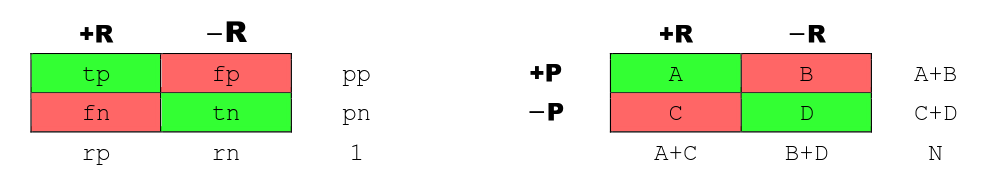
\includegraphics[width=0.8\textwidth]{Matriz_de_confusao.png}
    \fonte{\cite{POWERS2020}}
    \label{fig:Matriz_de_confusao}
\end{figure}

\subsubsection{\textit{Recall}}
Essa métrica relaciona a quantidade de verdadeiros positivos e falsos positivos do modelo e será referenciada como \textit{True Positive Rate} (\textit{tpr}), e é 
descrita como: 

\begin{equation}
    Recall = Sensitivity = tpr = tp/tr
           = TP / RP = A / (A + C)
\end{equation}

\subsubsection{Precisão}
Precisão denota a proporção de casos preditos positivos que foram preditos corretamente. Pode ser chamado também de Acurácia de verdadeiros positivos 
(\textit{True Positive Accuracy - TPA}). Precisão é definida por:

\begin{equation}
    Precision = Confidence = tpa = tp / pp
              = TP / PP = A / (A + B)
\end{equation}

\subsubsection{\textit{F1-Score}}
A medida F1 efetivamente relaciona a proporção de Verdadeiros Positivos (\textit{True Positives}) à média aritmética das previsões positivas (\textit{Predicted 
Positives}) e dos casos reais positivos (\textit{Real Positives}), é descrita como: 

\begin{equation}
    F1 = tp / (tp + (fn + fp) / 2)
       = A / (A + (B + C) / 2)
\end{equation}

\subsubsection{Generalização}
Apesar de inicialmente as métricas serem definidas para um modelo de classificação binária em seu trabalho \citeonline{POWERS2020} conclui que essas relações podem ser
generalizadas ao atender dois requisitos: 

\begin{itemize}
    \item Classes reais e classes previstas são categorizadas por $K$ rótulos
    \item Cada classe deve ser não vazia
\end{itemize}

É necessário ressaltar que, devido à natureza de alta frequência dos dados, a série de retornos discretizados 
apresentará um forte desbalanceamento de classes. Como apontado por \citeonline{jjfinec}, a grande maioria das observações está concentrada em movimentos
estatisticamente irrelevantes ou ruído (0). Por consequência, a Acurácia global e a Taxa de Erro, embora úteis para uma visão geral, 
podem apresentar valores artificialmente elevados caso o modelo adote um comportamento de persistência focado na classe majoritária. 
Para mitigar essa armadilha estatística e garantir a utilidade prática do modelo, a avaliação de desempenho priorizará a análise isolada das métricas de 
\textit{Precisão}, \textit{Recall} e \textit{F1-Score} especificamente para os rótulos de movimentação direcional (1 e -1). 
O modelo será considerado superior aos baselines apenas se demonstrar vantagem preditiva sobre esses estados significativos.

% ---------------------------------------------------------------
\section{Trabalhos relacionados}
\label{sec:trabalhos_relacionados}

\subsection{Trabalho 1: Reconstructing Cryptocurrency Processes via Markov Chains}
\label{sec:trabalho1_araujo}

O estudo de \citeonline{ARAUJO}, intitulado \textit{Reconstructing Cryptocurrency Processes via Markov Chains} e publicado no periódico \textit{Computational Economics 
(Springer Nature)}, possui forte alinhamento com os objetivos deste trabalho. A pesquisa busca reconstruir e prever os processos estocásticos de três das principais 
criptomoedas do mercado Bitcoin, Ethereum e Ripple, investigando a existência de componentes de memória de longo alcance em suas séries temporais \cite{ARAUJO}.

A motivação dos autores é tanto técnica quanto empírica. Eles constatam a inviabilidade estatística de utilizar livremente Cadeias de Markov de ordem elevada na 
predição de séries financeiras, uma vez que o número de combinações possíveis (blocos) cresce exponencialmente com o aumento da ordem, superando rapidamente o tamanho 
da amostra disponível.

Para contornar essas limitações, a análise é fundamentada em fechamentos intradiários de uma hora. Inicialmente, os autores utilizam um alfabeto discreto de cinco 
símbolos, construído com base na média ($\overline{r(t)}$) e no desvio padrão ($s$) dos retornos, estruturado da seguinte forma:

\begin{equation}
    \begin{aligned}
        (r(t) - \overline{r(t)}) > s &\iff 2 \\
        s \geq (r(t) - \overline{r(t)}) > \frac{s}{3} &\iff 1 \\
        \frac{s}{3} \geq (r(t) - \overline{r(t)}) > -\frac{s}{3} &\iff 0 \\
        -\frac{s}{3} \geq (r(t) - \overline{r(t)}) > -s &\iff -1 \\
        -s \geq (r(t) - \overline{r(t)}) &\iff -2
    \end{aligned}
    \label{eq:alfabeto_cinco_araujo}
\end{equation}

Mesmo com o alfabeto de cinco caracteres, observou-se que o crescimento exponencial inerente às cadeias de alta ordem compromete a viabilidade estatística do modelo 
para dimensões $k \geq 4$. Nesse ponto, o tamanho da amostra de treinamento torna-se inferior ao conjunto de possibilidades, o que faria o modelo falhar diante de 
sequências de observações inéditas. 

Para mitigar esse problema, \citeonline{ARAUJO} adotam a abordagem proposta por \citeonline{MENDES}, conhecida como \textit{Less-than-k-Markov}. Esse método recorre a 
probabilidades de matrizes de ordens menores $\{ k-1, k-2, k-3, ..., 2 \}$ de forma iterativa quando uma sequência específica de tamanho $k$ não é encontrada na amostra 
histórica.

\begin{figure}[htbp]
    \centering
    \caption{Comparação do número de ocorrências de sequências de tamanho $k$ para $5^k$.}
    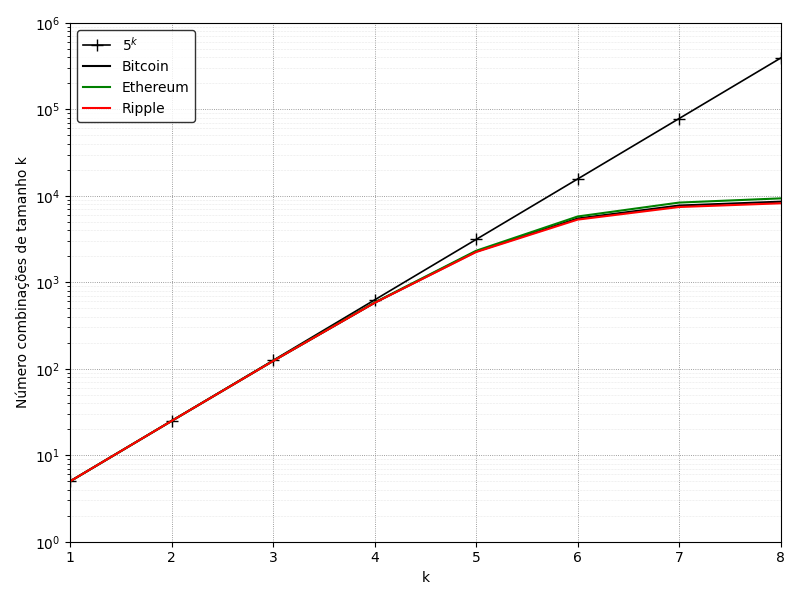
\includegraphics[width=0.8\textwidth]{images/grafico_kblocos.png}
    \fonte{\cite{ARAUJO}, adaptado pelos autores.}
    \label{fig:grafico_kblocos}
\end{figure}

Os autores concluem, através da análise de acurácia do modelo para o alfabeto de cinco símbolos, que o algoritmo performa consistentemente melhor em comparação ao 
modelo de predição aleatório para todas as criptomoedas utilizadas na análise, conforme ilustrado na Figura~\ref{fig:Araujo_cinco_simbolos}. Esse comportamento sugere 
que o componente de memória de curto prazo se manifesta de maneira robusta e similar no mercado de ativos digitais.

\begin{figure}[htbp]
    \centering
    \caption{Erro médio obtido na predição para $k$ dimensões e $5$ símbolos.}
    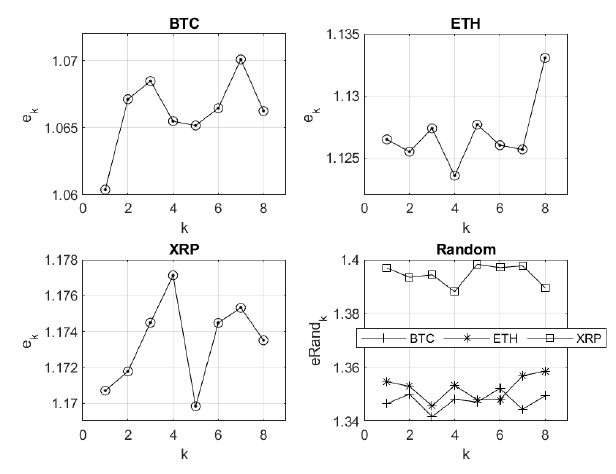
\includegraphics[width=0.8\textwidth]{images/Araujo_cinco_simbolos.png}
    \fonte{\cite{ARAUJO}}
    \label{fig:Araujo_cinco_simbolos}
\end{figure}

Influenciados pela necessidade de caracterizar de maneira mais satisfatória a presença de pequenas flutuações e ruídos, além de buscar uma melhora na estabilidade 
estatística do treinamento, os autores testaram uma segunda configuração utilizando um alfabeto discreto constituído de três símbolos

\begin{equation}
    \begin{aligned}
        (r(t) - \overline{r(t)}) > s &\iff 1 \\
        s \geq (r(t) - \overline{r(t)}) > -s &\iff 0 \\
        -s \geq (r(t) - \overline{r(t)}) &\iff -1
    \end{aligned}
    \label{eq:alfabeto_tres_araujo}
\end{equation}

Ao agrupar flutuações pouco expressivas em torno da média, essa estratégia desconsiderou ruídos irrelevantes de alta frequência. Como resultado, observou-se uma diminuição significativa nos erros obtidos na predição, estendendo a vantagem do modelo empírico para blocos de ordens maiores e preservando a identificação de componentes de memória de curto e longo alcance.

\begin{figure}[htbp]
    \centering
    \caption{Erro médio obtido na predição para $k$ dimensões e $3$ símbolos.}
    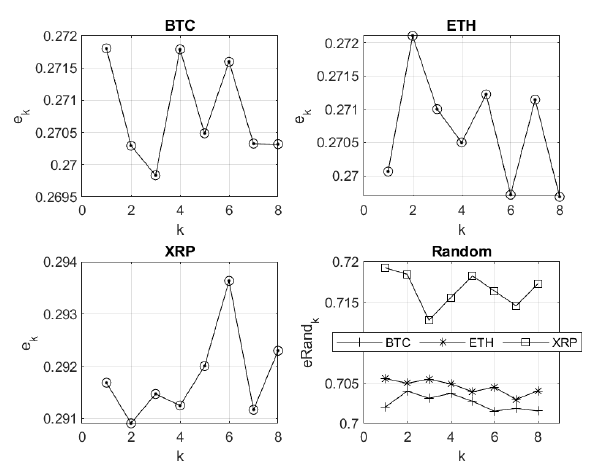
\includegraphics[width=0.8\linewidth]{images/Araujo_tres_simbolos.png}
    \fonte{\cite{ARAUJO}}
    \label{fig:Araujo_tres_simbolos}
\end{figure}

O presente trabalho utilizará um alfabeto discreto construído de maneira metodologicamente similar ao referencial de três símbolos conforme apresentado na Seção~\ref{discretizacao}. Porém, a análise intradia será realizada para uma escala de alta frequência, utilizando fechamentos em janelas de cinco minutos.

Para contornar a explosão combinatória e os limites computacionais que restringiram o avanço da ordem preditiva no estudo de \citeonline{ARAUJO}, esta pesquisa 
empregará a modelagem baseada em Cadeias de Markov de alta ordem proposta por \citeonline{RAFTERY1985}. A adoção deste modelo reduz a complexidade dos modelos de Markov de Alta 
Ordem, tornando viável a investigação de dependências temporais em ordens substancialmente maiores do que as apresentadas na literatura de referência, sem sacrificar a 
confiabilidade preditiva do sistema.

\subsection{Trabalho 2: Extracting Rules via Markov Chains for Cryptocurrencies Returns Forecasting}

O estudo de \citeonline{NASCIMENTO}, intitulado Extracting Rules via Markov Chains for Cryptocurrencies Returns Forecasting e publicado no periódico Computational 
Economics, possui forte alinhamento com os objetivos deste trabalho. Em sua pesquisa, os autores utilizam Cadeias de Markov de alta ordem para extrair regras das 
dinâmicas de retorno de quatro criptomoedas do mercado: Bitcoin, Ethereum, Litecoin e Ripple. O estudo analisou os preços diários de fechamento em dólar, no período de 
1º de outubro de 2016 a 30 de novembro de 2019, totalizando 1156 observações para cada ativo.

A principal motivação do estudo é determinar possíveis cenários futuros analisando a dependência de memória na dinâmica do processo, obtendo regras de transição de 
estados a partir das informações do conjunto de dados. Para isso, os autores constroem um modelo preditivo baseado nos retornos logarítmicos dos preços através da 
equação $r_t = log(z_t) - log(z_{t-1})$, onde $z_t$ corresponde ao valor observado no dia atual e $z_{t-1}$ ao valor observado no dia anterior.

Para realizar a análise, Nascimento descreve a necessidade de categorizar a série e enfatiza que a granularidade dos dados pode influenciar os resultados. Desse modo, 
foram testadas quatro granularidades (0,1; 0,01; 0,001 e 0,0001) com a finalidade de discretizar os retornos e encontrar o melhor ajuste para as séries temporais. 
Essas granularidades representam os intervalos numéricos onde a série será categorizada, sendo o escopo total definido entre o menor e o maior valor da série temporal, subtraindo e somando o valor da respectiva granularidade.

Uma vez que a série temporal é classificada, os autores definem os estados de transição da matriz de forma que o número de estados para cada granularidade seja equivalente ao número total de categorias menos um. Como exemplo, para a série do Bitcoin com granularidade 0,1, o intervalo de categorização obtido foi de $[-0{,}286095194;\ 0{,}324052773]$. Nesse cenário, foram geradas seis categorias, resultando em cinco possíveis estados para a matriz de transição.

Para validar o modelo, o estudo utilizou três métricas: a Raiz do Erro Quadrático Médio, do inglês \textit{Root Mean Square Error} (RMSE), o Erro Médio Absoluto, do inglês \textit{Mean Absolute Error} (MAE) e o Erro Percentual Absoluto Médio, do inglês \textit{Mean Absolute Percentage Error} (MAPE). O RMSE e o MAE foram utilizados para determinar qual ordem da Cadeia de Markov obteve a melhor acurácia dentro de cada granularidade, enquanto o MAPE auxiliou na escolha da granularidade ideal. Nascimento conclui que, para o Bitcoin, um processo de Markov na sétima ordem produz os melhores resultados, corroborando a hipótese de que as séries temporais de criptomoedas possuem memória de longo alcance.

O presente trabalho também utilizará processos de Markov de alta ordem e também modelos ocultos de Markov, porém com foco em modelos preditivos direcionais. Para isso, será adotado um alfabeto constituído por três símbolos, diferindo metodologicamente do estudo de Nascimento, que utilizou intervalos contínuos baseados em granularidade. A adoção de um alfabeto discreto e reduzido evita o problema de explosão de estados e complexidade computacional encontrado por \citeonline{NASCIMENTO} em granularidades muito baixas. Como o objetivo desta pesquisa difere da predição de valores absolutos, a validação dos modelos direcionais será feita por meio de métricas adequadas a problemas de classificação, tais como Matriz de Confusão, Acurácia, Precisão e F1-Score. Por fim, a janela de tempo analisada também se difere do fechamento diário utilizado na literatura supracitada; com base nas observações de \citeonline{GONZALEZ2025}, este trabalho adotará janelas de fechamento de cinco minutos, consideradas mais adequadas para a análise de séries temporais do Bitcoin.

\subsection{Trabalho 3: Bitcoin price prediction using machine learning: An approach
to sample dimension engineering}

O estudo de \citeonline{CHEN}, intitulado \textit{Bitcoin price prediction using machine learning: An approach
to sample dimension engineering} e publicado no periódico \textit{Journal of Computational and Applied Mathematics}, possui forte alinhamento com os objetivos deste trabalho. Em seu trabalho \citeonline{CHEN} busca definir os melhores métodos de aprendizado de máquina para predição de preços para o Bitcoin. \citeonline{CHEN} divide a amostra de predição em uma amostra pequena de fechamentos diários e uma amostra maior de fechamento de 5 minutos. Os autores expressam que essa decisão se deve à estrutura diferente dos dados e que aplicar modelos de aprendizado de máquina de forma incorreta gera um erro nos modelos chamado sobreajuste (\textit{overfitting}). Então os autores empregam modelos estatísticos para o fechamento diário do preço do Bitcoin, enquanto utilizam de métodos de aprendizado de máquina para a amostra de alta frequência, ou seja, fechamentos de cinco minutos. 

Além da preocupação com a dimensionalidade da amostra, os autores transformam o desafio preditivo em um problema de classificação binária, focando exclusivamente em prever a direção (mudança de sinal) do preço do ativo. A justificativa é que a predição direcional é mais prática para fundamentar decisões de negociação no mercado financeiro. Por se tratar de um problema de classificação direcional, o desempenho dos modelos foi validado por meio de uma Matriz de Confusão e métricas específicas, como Acurácia, Precisão, \textit{Recall} e F1-Score. 

O presente trabalho corrobora a utilidade da janela de cinco minutos para capturar as dinâmicas de alta frequência e adota o foco direcional estabelecido por \citeonline{CHEN}, outro ponto em comum é a utilização de um alfabeto para classificar a série temporal, que no presente trabalho é um alfabeto composto por três símbolos diferindo-se da metodologia de \citeonline{CHEN}, o presente trabalho também utilizará das métricas empregadas pelos autores com a finalidade de validar os modelos empregados. Contudo, diferentemente do uso de algoritmos de aprendizado de máquina em larga escala, esta pesquisa se propõe a modelar o comportamento direcional do Bitcoin utilizando Cadeias de Markov de alta ordem e modelos ocultos de Markov. Essa abordagem estocástica permite extrair a dependência temporal e as regras de transição inerentes aos retornos de cinco minutos de forma clara, reduzindo a complexidade computacional exigida por modelos tradicionais de aprendizado de máquina, ao mesmo tempo em que mantém o rigor na avaliação preditiva através do uso das métricas de classificação adequadas. 

\subsection{Síntese Comparativa}

A análise individual de cada um dos trabalhos relacionados permite compreender com maior clareza o posicionamento desta pesquisa no cenário acadêmico atual, bem como suas diferenças em relação às abordagens comumente adotadas na literatura. A Tabela \ref{tab:tabela_um} sintetiza os principais pontos de divergência entre os trabalhos analisados e as metodologias empregadas por seus respectivos autores.

\begin{table}[htb]
    \centering
    \caption{Comparação entre trabalhos relacionados.}
    \label{tab:tabela_um}
    \footnotesize
    \renewcommand{\arraystretch}{1.25}
    \setlength{\tabcolsep}{4pt}
        \begin{tabularx}{\textwidth}{%
            >{\raggedright\arraybackslash}p{1.7cm}%
            >{\raggedright\arraybackslash}X%
            >{\raggedright\arraybackslash}X%
            >{\raggedright\arraybackslash}X%
            >{\raggedright\arraybackslash}X}
        \toprule
        \textbf{Critério} & \textbf{Araújo e Barbosa (2024)} & \textbf{Nascimento (2023)} & \textbf{Chen (2025)} & \textbf{Este trabalho} \\
        \midrule
        Objetivo & Reconstruir processos de criptoativos e detectar memória de longo alcance & Prever retornos futuros de quatro criptomoedas via Cadeias de Markov & Prever a direção do preço do Bitcoin comparando algoritmos de \textit{ML} & Prever a direção do BTC e identificar a ordem em que a memória se torna relevante \\
        \addlinespace
        Ativos & Bitcoin, Ethereum e Ripple & Bitcoin, Ethereum, Ripple e Litecoin & Bitcoin & Bitcoin \\
        \addlinespace
        Fechamento   & 1 hora & 24 horas & Diária e intradiária (5 min) & Intradiária (5 min) \\
        \addlinespace
        Modelagem & Cadeias de Markov de alta ordem (\textit{less-than-k}) & Cadeias de Markov (1ª à 10ª ordem) & Regressão logística, LDA, QDA, SVM, XGBoost e LSTM & Cadeias de Markov de alta ordem (MTD/Raftery) e HMM \\
        \addlinespace
        Discretização & Alfabetos de 5 e 3 símbolos & Múltiplos alfabetos & Binária (direção) & Alfabeto de 3 símbolos (limiares $s/3$, $s/4$, $s/5$) \\
        \addlinespace
        Validação & Erro médio \textit{vs.} modelo aleatório & RMSE, MAE e MAPE & Acurácia, precisão, \textit{recall} e \textit{F1-score} & Acurácia, precisão, \textit{recall}, F1 e matriz de confusão \textit{vs.} \textit{baselines} \\
        \addlinespace
        Limitação & Explosão combinatória limita a ordem ($k \geq 4$) & Memória limita a análise até a 10ª ordem & Granularidade e número de dimensões & --- \\
        \bottomrule
        \end{tabularx}
    \par\vspace{2pt}
    \footnotesize Fonte: Elaborado pelos autores (2026).
\end{table}

% ===============================================================
% CAPÍTULO 3 - DESENVOLVIMENTO
% ===============================================================
\chapter{Desenvolvimento}
\label{cap:desenvolvimento}

Este capítulo apresenta o desenvolvimento metodológico desta pesquisa,
detalhando os passos fundamentais executados para alcançar o objetivo principal do projeto.
Sendo o foco estruturar a solução proposta, a seção descreve como foram conduzidas
a coleta de dados, a modelagem preditiva baseada em Cadeias de Markov de Alta Ordem
e Modelos Ocultos de Markov, do inglês \textit{Hidden Markov Model} (HMM), e a avaliação de desempenho. Todas as decisões
tecnológicas e arquiteturais adotadas na etapa de implementação foram fundamentadas
na revisão bibliográfica discutida no Capítulo \ref{cap:revisao}.

% ---------------------------------------------------------------
% ---------------------------------------------------------------
\section{Visão geral da solução}

A solução proposta consiste em um conjunto de modelos que preveem o próximo símbolo da série discretizada do Bitcoin, 
em janelas de cinco minutos, a partir dos símbolos anteriores. Duas famílias de modelos são avaliadas, Cadeias de Markov de alta ordem, 
segundo a formulação de Mistura de Distribuições de Transição (MTD) proposta por \citeonline{RAFTERY1985}, 
ajustadas com ordens de 1 a 10; e os Modelos Ocultos de Markov (HMM), ajustados com 2 a 5 estados ocultos 
pelo algoritmo de Baum-Welch.

Para verificar se esses modelos oferecem ganho preditivo real, seu desempenho é 
comparado ao de quatro modelos de referência:

\begin{itemize}
    \item o modelo aleatório, que sorteia um dos três símbolos com probabilidades iguais;
    \item o modelo de persistência, que prevê a repetição do último símbolo observado;
    \item o modelo de frequências, que atribui a cada símbolo a sua proporção no conjunto de treinamento, sem considerar o passado;
    \item a cadeia de Markov de primeira ordem, que considera apenas o símbolo imediatamente anterior.
\end{itemize}

Todos os modelos operam sobre a mesma série discreta, obtida pela discretização 
dos retornos logarítmicos em um alfabeto de três símbolos ($-1$, $0$ e $1$) com limiar adaptativo, 
conforme a estratégia apresentada na Seção \ref{discretizacao}. 
A sensibilidade dos resultados à discretização é avaliada com os limiares $s/4$ e $s/5$ e com o limiar fixo. 
Os modelos são ajustados sobre o conjunto de treinamento e avaliados sobre o conjunto de teste, 
sempre prevendo um passo à frente com base apenas nos símbolos anteriores.

A avaliação segue o critério definido na Seção \ref{avaliacao}: matriz de confusão, precisão, 
\textit{recall} e F1 das classes direcionais ($-1$ e $1$). 

Essas métricas são complementadas pela log-verossimilhança e pela AUC, que avaliam as probabilidades 
previstas sem depender da regra de decisão adotada.

\section{Pipeline da solução}

\begin{itemize}

    \item \textbf{Coleta dos dados}: Os dados históricos foram coletados a partir da \textit{exchange Binance}, focando especificamente no par
    de negociação BTC/USD. A amostragem consistiu no preço de fechamento em janelas de cinco minutos, abrangendo um período de nove anos e
    totalizando aproximadamente 920 mil registros.

    \item \textbf{Limpeza e Tratamento de Dados Ausentes}: Visando garantir a reprodutibilidade e a integridade estatística da série,
    utilizou-se uma etapa de pré-processamento. Janelas temporais faltantes (\textit{gaps}) geradas por falhas de registro ou
    períodos de manutenção da corretora foram identificadas. Para evitar a geração de retornos logarítmicos errados devido a saltos temporais,
    adotou-se o descarte das observações no momento da falha. Dessa forma, o cálculo de retorno ocorreu exclusivamente entre janelas de cinco
    minutos consecutivas. Valores discrepantes (\textit{outliers}) decorrentes de anomalias de registro também foram descartados nesta etapa.

    \item \textbf{Tratamento e discretização dos dados}: Os dados foram discretizados utilizando
    a estratégia apresentada na Seção~\ref{discretizacao}, obtendo-se assim uma nova série temporal de
    símbolos pertencentes ao alfabeto simbólico, a qual foi repartida em conjunto
    de treinamento e teste.

    \item \textbf{Separação dos Dados Históricos}:
    Considerando a evolução estrutural de criptoativos
    que os fez sair de um nicho tecnológico para um fenômeno financeiro global \cite{MAKAROV2022},
    foi realizada a divisão do conjunto de dados em subamostras. Como as séries financeiras
    naturalmente apresentam quebras estruturais, alternando entre fases de alta, baixa e
    lateralização que afastam a propriedade de estacionariedade em  longas janelas de tempo \cite{morettin2018analise}, o intuito
    dessa divisão foi mitigar um possível viés de homogeneidade.

    \item \textbf{Treinamento e adequação dos Modelos Preditivos}: O conjunto de treinamento discretizado foi utilizado
    para alimentar e ajustar as Cadeias de Markov e o modelo HMM.

    \item \textbf{Testes Estatísticos, Comparações e Predição}: Os modelos de predição já treinados realizaram as predições
    sobre o conjunto de dados separado para os testes. A adequação dos modelos foi avaliada através dos métodos estatísticos
    descritos na Seção~\ref{avaliacao}. De forma crucial para a validação da hipótese deste estudo, a superação dos modelos empíricos
    (aleatório e persistência) não foi medida apenas pela taxa de acerto global, mas pela capacidade da
    matriz de confusão e do F1-Score em atestar a correta predição das classes (1 e -1), que representam os movimentos direcionais de interesse.

\end{itemize}

\begin{figure}[htbp]
    \centering
    \caption{Pipeline da solução proposta.}
    \label{fig:pipeline}
    \resizebox{\textwidth}{!}{%
    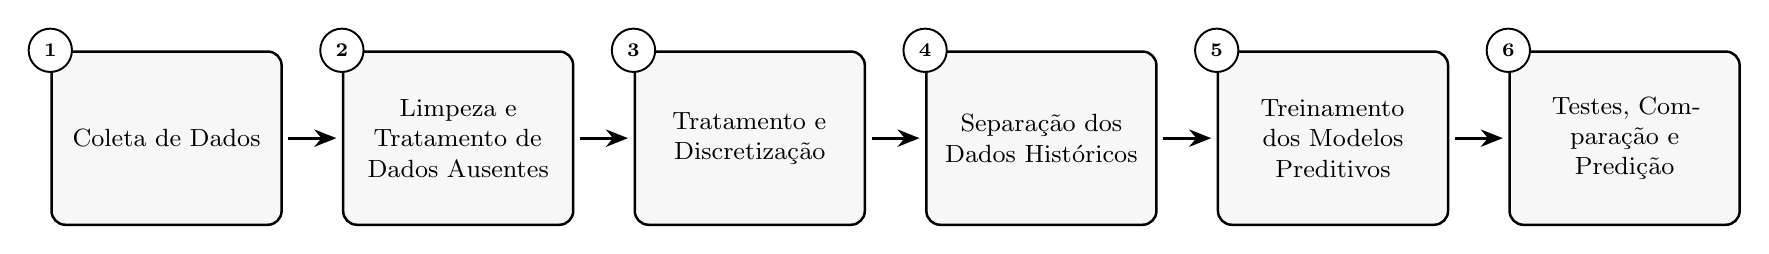
\begin{tikzpicture}[
        node distance=0.75cm,
        pbox/.style={
            rectangle,
            rounded corners=5pt,
            draw=black,
            line width=0.9pt,
            fill=gray!6,
            text width=2.5cm,
            align=center,
            minimum height=2.2cm,
            font=\small,
            inner sep=6pt
        },
        pnum/.style={
            circle,
            draw=black,
            fill=white,
            line width=0.7pt,
            minimum size=0.55cm,
            inner sep=0pt,
            font=\scriptsize\bfseries
        },
        arrow/.style={
            line width=1pt,
            -{Stealth[length=2.8mm, width=2.2mm]},
            shorten >=2pt,
            shorten <=2pt
        }
        ]

        \node (p1) [pbox] {Coleta de Dados};
        \node (p2) [pbox, right=of p1] {Limpeza e Tratamento de Dados Ausentes};
        \node (p3) [pbox, right=of p2] {Tratamento e Discretização};
        \node (p4) [pbox, right=of p3] {Separação dos Dados Históricos};
        \node (p5) [pbox, right=of p4] {Treinamento dos Modelos Preditivos};
        \node (p6) [pbox, right=of p5] {Testes, Comparação e Predição};

        \node [pnum] at (p1.north west) {1};
        \node [pnum] at (p2.north west) {2};
        \node [pnum] at (p3.north west) {3};
        \node [pnum] at (p4.north west) {4};
        \node [pnum] at (p5.north west) {5};
        \node [pnum] at (p6.north west) {6};

        \draw [arrow] (p1) -- (p2);
        \draw [arrow] (p2) -- (p3);
        \draw [arrow] (p3) -- (p4);
        \draw [arrow] (p4) -- (p5);
        \draw [arrow] (p5) -- (p6);

    \end{tikzpicture}
    }
    \fonte{Elaborado pelos autores (2026).}
\end{figure}

% ---------------------------------------------------------------
\section{Arquitetura e coleta de dados}
\label{sec:arquitetura}

A solução é organizada em duas partes, ilustradas na Figura~\ref{fig:arquitetura}. A primeira é um serviço de coleta que mantém uma base de 
dados histórica sempre atualizada. A segunda é o ambiente de experimentos, que trabalha sobre uma cópia congelada dessa base para que os 
resultados possam ser reproduzidos.

\begin{figure}[htbp]
    \centering
    \caption{Arquitetura da solução: coleta contínua e ambiente de experimentos.}
    \label{fig:arquitetura}
    \resizebox{\textwidth}{!}{%
    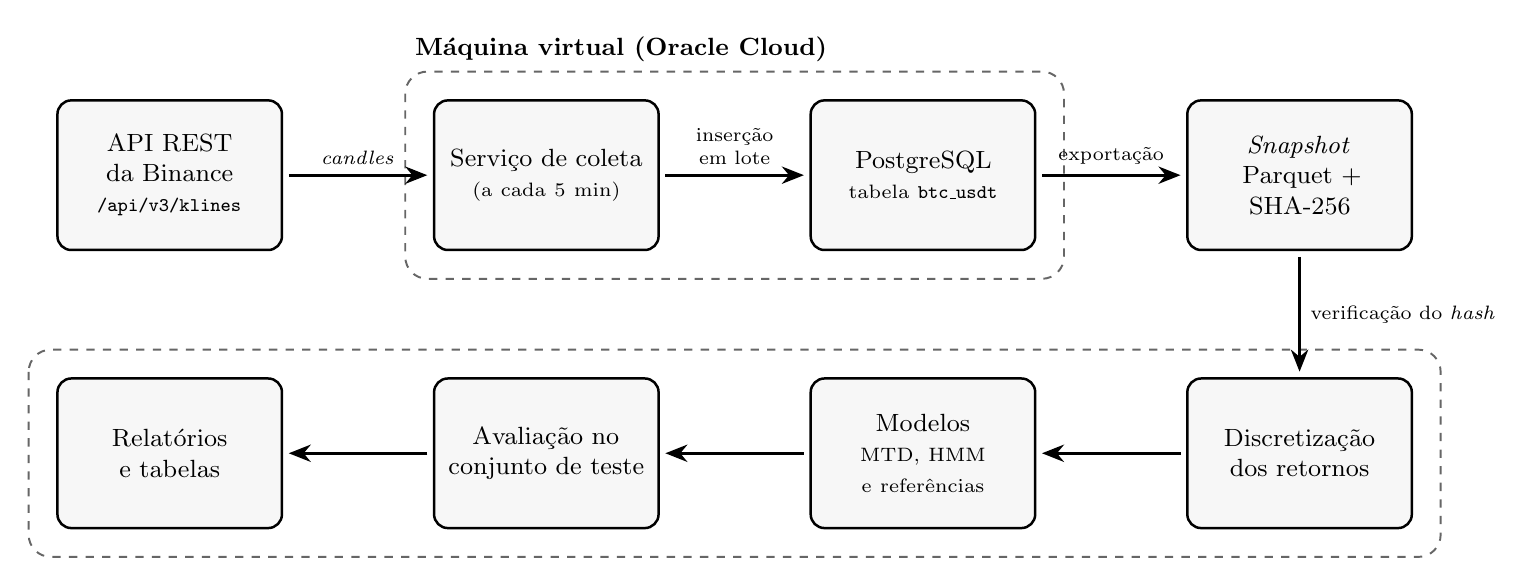
\begin{tikzpicture}[
        node distance=0.6cm and 1.9cm,
        abox/.style={
            rectangle,
            rounded corners=5pt,
            draw=black,
            line width=0.9pt,
            fill=gray!6,
            text width=2.5cm,
            align=center,
            minimum height=1.9cm,
            font=\small,
            inner sep=5pt
        },
        zona/.style={
            rounded corners=8pt,
            draw=black!60,
            dashed,
            line width=0.7pt
        },
        rotulo/.style={
            font=\small\bfseries,
            anchor=south west
        },
        arrow/.style={
            line width=1pt,
            -{Stealth[length=2.8mm, width=2.2mm]},
            shorten >=2pt,
            shorten <=2pt
        },
        legenda/.style={
            font=\scriptsize,
            midway,
            fill=white,
            inner sep=1.5pt,
            align=center
        }
        ]

        % Coleta (linha superior)
        \node (api) [abox] {API REST da Binance\\ \scriptsize\texttt{/api/v3/klines}};
        \node (coleta) [abox, right=of api] {Serviço de coleta\\ \scriptsize(a cada 5 min)};
        \node (banco) [abox, right=of coleta] {PostgreSQL\\ \scriptsize tabela \texttt{btc\_usdt}};
        \node (snap) [abox, right=of banco] {\textit{Snapshot}\\ Parquet + SHA-256};

        % Experimentos (linha inferior, da direita para a esquerda)
        \node (disc) [abox, below=1.6cm of snap] {Discretização dos retornos};
        \node (modelos) [abox, left=of disc] {Modelos\\ \scriptsize MTD, HMM e referências};
        \node (aval) [abox, left=of modelos] {Avaliação no conjunto de teste};
        \node (rel) [abox, left=of aval] {Relatórios e tabelas};

        % Zonas (retângulos tracejados desenhados a partir dos cantos das caixas)
        \draw [zona] ([xshift=-0.35cm, yshift=0.35cm]coleta.north west)
            rectangle ([xshift=0.35cm, yshift=-0.35cm]banco.south east);
        \node [rotulo] at ([xshift=-0.35cm, yshift=0.35cm]coleta.north west) {Máquina virtual (Oracle Cloud)};
        \draw [zona] ([xshift=-0.35cm, yshift=0.35cm]rel.north west)
            rectangle ([xshift=0.35cm, yshift=-0.35cm]disc.south east);

        % Fluxo
        \draw [arrow] (api) -- node[legenda, above=2pt, fill=none] {\textit{candles}} (coleta);
        \draw [arrow] (coleta) -- node[legenda, above=2pt, fill=none] {inserção\\em lote} (banco);
        \draw [arrow] (banco) -- node[legenda, above=2pt, fill=none] {exportação} (snap);
        \draw [arrow] (snap) -- node[legenda, right=2pt, fill=none] {verificação do \textit{hash}} (disc);
        \draw [arrow] (disc) -- (modelos);
        \draw [arrow] (modelos) -- (aval);
        \draw [arrow] (aval) -- (rel);

    \end{tikzpicture}
    }
    \fonte{Elaborado pelos autores (2026).}
\end{figure}

\subsection{Fonte dos dados}

Os dados históricos foram obtidos da \textit{exchange} Binance, por meio do \textit{endpoint} público \texttt{/api/v3/klines} 
da sua API REST \cite{BINANCE_API}. Foram coletados os \textit{candles} de cinco minutos do par BTC/USDT, isto é, o preço do Bitcoin 
cotado em Tether (USDT), uma criptomoeda pareada ao dólar americano. Cada \textit{candle} resume as negociações de um intervalo 
de cinco minutos e contém, entre outros campos, o instante de abertura, os preços de abertura, máxima, mínima e fechamento, o volume 
negociado e o número de negociações. Neste trabalho, apenas o preço de fechamento é utilizado para calcular os retornos.

A coleta parte do primeiro \textit{candle} disponível para o par, em 17 de agosto de 2017. Cada requisição devolve no máximo 1.000 \textit{candles}, 
de modo que o histórico é obtido em requisições sucessivas, cada uma a partir do último instante já recebido. Em caso de falha de rede ou 
de limite de requisições da API, a requisição é repetida até cinco vezes, com intervalos crescentes entre as tentativas (de 1 a 60 segundos).

\subsection{Armazenamento e coleta contínua}

Os \textit{candles} são armazenados em um banco de dados PostgreSQL hospedado em uma máquina virtual na Oracle. A tabela \texttt{btc\_usdt} 
guarda as colunas originais da API e tem como chave primária o instante de abertura do \textit{candle}, junto com o par e o intervalo, 
já que a própria API identifica cada \textit{candle} pelo seu instante de abertura \cite{BINANCE_API}. A inserção é feita em lotes: os \textit{candles} 
de cada requisição são carregados em uma tabela temporária e depois copiados para a tabela definitiva, ignorando os que já existem. 
Assim, uma mesma janela de tempo pode ser coletada mais de uma vez sem gerar registros duplicados.

Um serviço executado continuamente na mesma máquina mantém a base atualizada. A cada cinco minutos, 
ele consulta o instante do último \textit{candle} armazenado e solicita à API apenas os que ainda faltam. O acesso ao banco a partir de 
outras máquinas é feito exclusivamente por um túnel SSH, de modo que o banco não fica exposto diretamente à internet.


\section{Detalhes da implementação}
\label{sec:implementacao}

Esta seção detalha toda a implementação desenvolvida neste trabalho.

% 3.3.1
\subsection{Lacunas e segmentos contínuos}
\label{subsec:lacunas}
Como explicado na coleta de dados, nossa fonte, a API da Binance, pode apresentar perda de dados. Para garantir a 
reprodutibilidade dos experimentos, fixamos um período de dados, que chamamos de \textit{snapshot} e detalhamos na 
Seção~\ref{subsec:ambiente}. A \textit{snapshot} usada neste estudo contém os dados 
disponíveis via API da Binance de 2017-08-17 04:00 até 2026-09-30 23:55, e as métricas observadas nesse período estão na 
Tabela~\ref{tab:lacunas}.

\begin{table}[htb]
  \centering
  \caption{\textit{Candles}, lacunas e segmentos da \textit{snapshot}}
  \label{tab:lacunas}
  \begin{tabular}{lr}
    \toprule
    Grandeza & Valor \\
    \midrule
    \textit{Candles} na \textit{snapshot} & 957.853 \\
    Lacunas & 34 \\
    \textit{Candles} faltantes & 1.715 \\
    Segmentos contínuos & 35 \\
    \bottomrule
  \end{tabular}
  \legend{Fonte: Elaborado pelos autores (2026).}
\end{table}

\begin{itemize}
\item \textit{Candle}: registro de um intervalo de 5 minutos.
\item \textit{Lacuna}: ausência de pelo menos um \textit{candle} entre um horário de captura e o próximo.
\item \textit{Segmento}: sequência contínua de capturas, delimitada por lacunas.
\end{itemize}

As lacunas e os segmentos são fundamentais para uma discretização correta, pois ignorar as lacunas levaria a tratar retornos 
de intervalos superiores a 5 minutos como se fossem retornos de 5 minutos. Por exemplo: imagine que a API da Binance tenha 
ficado fora do ar das 10:30 às 11:30 UTC. Se a captura das 10:30 registrou o valor de fechamento 61.130.48USD\$ e a das 11:30, já com a API de volta, 
registrou o valor 61.131.42USD\$, não é correto calcular o retorno entre esses dois valores na discretização, pois o retorno de 10:30 para 
11:30 não é válido. Nesse caso, há uma lacuna das 10:35 às 11:25 e, portanto, dois segmentos nesse dia.

% 3.3.2 
\subsection{Retorno e Limiares}
\label{subsec:retorno}

Em nossa discretização, calculamos o retorno logarítmico (Equação~\ref{retorno_logaritmico}) sobre a lista de \textit{candles}, 
comparando sempre o \textit{candle} atual com o anterior. Assim, o primeiro \textit{candle} de cada segmento não gera retorno, 
por não possuir um \textit{candle} anterior. O retorno só é calculado entre \textit{candles} consecutivos. Portanto, um retorno 
que atravessa dois segmentos, não é gerado (Seção~\ref{subsec:lacunas}).

Categorizamos os retornos pela Equação~\ref{discretizacao_eq}, com corte $s/k$, em que $k$ é um parâmetro inteiro. 
Nosso principal limiar é $s/3$. Notamos, em um de nossos trabalhos de referência \cite{ARAUJO}, uma lacuna: o uso de um único 
limiar para a discretização em três símbolos. Para suprir essa lacuna, empregamos neste trabalho diferentes limiares, o que 
permite comparar o desempenho dos modelos em cada discretização.

A Tabela~\ref{tab:distribuicao} 
apresenta a distribuição dos símbolos nos dois modos de discretização (Seção~\ref{subsec:discretizacao}). 
Observa-se nela que o parâmetro $k$ controla a largura da faixa do símbolo 0. Quanto maior o $k$, mais estreita é a faixa e 
menor é a proporção de símbolos 0. No modo \textit{Blocks}, por exemplo, com $k = 3$ temos uma proporção considerável de símbolos 
0, cerca de 42\%, e essa proporção diminui à medida que $k$ aumenta.

\begin{table}[htb]
  \centering
  \caption{Distribuição percentual dos símbolos, em \%, por modo de discretização e limiar}
  \label{tab:distribuicao}
  \resizebox{\textwidth}{!}{%
  \begin{tabular}{llrccc@{\hspace{1.5em}}ccc@{\hspace{1.5em}}ccc}
    \toprule
    \multirow{2}{*}{Modo} & \multirow{2}{*}{Limiar} & \multirow{2}{*}{Símbolos} & \multicolumn{3}{c}{Geral} & \multicolumn{3}{c}{Treino} & \multicolumn{3}{c}{Teste} \\
    \cmidrule(lr){4-6} \cmidrule(lr){7-9} \cmidrule(lr){10-12}
     &  &  & $-1$ & $0$ & $+1$ & $-1$ & $0$ & $+1$ & $-1$ & $0$ & $+1$ \\
    \midrule
    \textit{Blocks} & $s/3$ & 953.547 & 28,77 & 42,41 & 28,82 & 28,78 & 42,33 & 28,89 & 28,57 & 43,83 & 27,61 \\
    \textit{Blocks} & $s/4$ & 953.547 & 33,21 & 33,51 & 33,28 & 33,23 & 33,41 & 33,36 & 32,84 & 35,36 & 31,80 \\
    \textit{Blocks} & $s/5$ & 953.547 & 36,15 & 27,64 & 36,22 & 36,17 & 27,53 & 36,29 & 35,67 & 29,56 & 34,77 \\
    \midrule
    \textit{Global} & $s/3$ & 957.818 & 23,98 & 51,87 & 24,15 & 24,39 & 51,02 & 24,58 & 16,18 & 67,96 & 15,85 \\
    \textit{Global} & $s/4$ & 957.818 & 28,86 & 42,15 & 28,98 & 29,25 & 41,35 & 29,41 & 21,62 & 57,45 & 20,94 \\
    \textit{Global} & $s/5$ & 957.818 & 32,27 & 35,36 & 32,37 & 32,62 & 34,61 & 32,76 & 25,59 & 49,59 & 24,82 \\
    \bottomrule
  \end{tabular}%
  }
  \legend{Fonte: Elaborado pelos autores (2026).}
\end{table}

% 3.3.3
\subsection{Modos de discretização: \textit{Global} e \textit{Blocks}}
\label{subsec:discretizacao}

Neste estudo decidimos usar dois modos de discretização. No modo \textit{Global}, a média e o desvio padrão $s$ são calculados 
uma única vez, sobre todos os dados de treinamento, e usados na discretização de toda a série (Seção~\ref{subsec:retorno}).

O modo \textit{Blocks} parte da ideia de que a série do Bitcoin muda muito com o tempo e, portanto, não é estacionária (Seção~\ref{subsubsec:estacionariedade}), sendo motivado por trabalhos de 
normalização adaptativa \cite{URETTINI2024}. Nele, os dados são agrupados em blocos consecutivos de $n$ meses e a média e o desvio padrão são calculados 
para cada bloco. Os retornos de um bloco são classificados com as estatísticas do bloco anterior, de modo que nenhum símbolo é 
classificado com informação posterior a ele. Em nossos experimentos principais usamos $n = 1$, e também variamos $n$ em 2, 3, 6 
e 12 meses. A escolha de $n$ é um compromisso: blocos longos sofrem de não estacionariedade interna, e blocos curtos produzem 
estimativas ruidosas \cite{URETTINI2024}.

O modo \textit{Blocks} tem duas consequências. A primeira é que o primeiro bloco serve apenas para estimar as estatísticas do bloco 
seguinte e não gera símbolos. Com $n = 1$ perdemos o primeiro mês (agosto de 2017), e essa perda cresce com $n$. O conjunto de 
treinamento passa de 905.654 símbolos, com $n = 1$, para 810.244, com $n = 12$. A segunda é que os retornos do conjunto de teste 
não dependem exclusivamente do conjunto de treinamento, uma vez que um bloco já presente no conjunto de teste pode categorizar 
o bloco seguinte, também presente no conjunto de teste. Isso não utiliza informação futura, apenas dados já disponíveis naquele 
momento, e difere do modo \textit{Global}, em que o teste é discretizado exclusivamente com estatísticas do treinamento.

A Tabela~\ref{tab:distribuicao} mostra 
por que mantivemos os dois modos. No modo \textit{Global} com limiar $s/3$, a proporção de símbolos 0 passa de 51,02\% no 
treinamento para 67,96\% no teste, porque a volatilidade do período de teste é menor que a média do treinamento. No modo 
\textit{Blocks}, com o mesmo limiar, passa de 42,33\% para 43,83\%. Isso é coerente com a literatura de normalização adaptativa, 
segundo a qual estatísticas estimadas no treinamento só bastam quando a série é estacionária \cite{URETTINI2024}.

%3.3.4
\subsection{Divisão treino e teste}
\label{subsec:divisao}

Para nossos experimentos seguimos a proporção de treino e teste usada por \citeonline{Nascimento2023}, onde 95\% dos dados são usados para 
treinar os modelos, e 5\% são usados para testá-los. A divisão é cronológica, sem embaralhamento, e o corte é feito sobre os
\textit{candles}, antes do cálculo dos retornos. O modo de discretização afeta diretamente o tamanho do conjunto de treino.
Na Seção~\ref{subsec:discretizacao} destacamos como a discretização por blocos é feita. Uma de suas características é usar as
estatísticas do bloco anterior para categorizar os retornos do bloco atual. Desta forma, o primeiro bloco não possui símbolos e
serve apenas para categorizar o bloco seguinte. Por este motivo, ao aumentar o número de meses de cada bloco perdemos parte do
conjunto de treino, enquanto o conjunto de teste permanece com o mesmo tamanho. A Tabela~\ref{tab:divisao} mostra essa proporção
para diferentes tamanhos de bloco.

\begin{table}[htb]
  \centering
  \caption{Proporção entre treino e teste, em número de símbolos, por modo de discretização e intervalo de atualização $n$ (idêntica para todo $k$ de 1 a 10)}
  \label{tab:divisao}
  \begin{tabular}{llrrrrr}
    \toprule
    Modo & $n$ (meses) & Treino & Teste & Total & Treino (\%) & Teste (\%) \\
    \midrule
    \textit{Global} & --- & 909.925 & 47.893 & 957.818 & 95,00 & 5,00 \\
    \midrule
    \textit{Blocks} & 1 & 905.654 & 47.893 & 953.547 & 94,98 & 5,02 \\
    \textit{Blocks} & 2 & 897.098 & 47.893 & 944.991 & 94,93 & 5,07 \\
    \textit{Blocks} & 3 & 888.170 & 47.893 & 936.063 & 94,88 & 5,12 \\
    \textit{Blocks} & 6 & 861.723 & 47.893 & 909.616 & 94,73 & 5,27 \\
    \textit{Blocks} & 12 & 810.244 & 47.893 & 858.137 & 94,42 & 5,58 \\
    \bottomrule
  \end{tabular}
  \legend{Fonte: Elaborado pelos autores (2026).}
\end{table}

O modo \textit{Global}, por sua vez, não perde símbolos além dos retornos inexistentes (o primeiro \textit{candle} e as lacunas,
Seção~\ref{subsec:lacunas}), pois todos os retornos válidos são convertidos em símbolos. Por isso a proporção de 95\% e 5\% é
praticamente exata, já que o corte é feito sobre os \textit{candles}.

%3.4.1
\subsection{Modelos de referência}
\label{subsec:modelos_ref}

Neste trabalho chamamos de modelos de referência os seguintes modelos:

\begin{itemize}
  \item Markov de primeira ordem: uma matriz de transição simples olhando para o estado imediatamente anterior.
  \item Modelo de persistência: o modelo de persistência escolhe sempre a mesma constante, $-1$, $0$ ou $+1$.
  \item Modelo aleatório: atribui probabilidade $1/3$ a cada símbolo, independentemente do estado anterior.
\end{itemize}

Em nossos experimentos usamos principalmente o modelo de persistência para comparação com os modelos-alvo do trabalho. O modelo de persistência
é usado na comparação com a sua melhor constante. Por exemplo, suponha que, ao prever apenas a direção do movimento, o modelo que
escolhe sempre $+1$ (o preço sempre sobe) atinja um acerto de 46,2\%, enquanto o que escolhe sempre $-1$ (o preço sempre cai)
atinja 50,7\%. Neste caso, usaremos como referência a constante de maior acerto.

Em nossos relatórios buscamos responder duas perguntas:

\begin{enumerate}
  \item Haverá uma movimentação significante no mercado? 
  \item Se houver uma movimentação significante, qual o sinal dela?
\end{enumerate}

Movimentações significantes são todas as movimentações que ficam acima ou abaixo do nosso limiar empregado na discretização. O modelo de persistência é muito 
utilizado em nossos experimentos para ajudar a comparar nossos modelos-alvo na segunda pergunta. As perguntas respondidas e os resultados dos experimentos serão 
detalhados na Seção~\ref{sec:resultados}.

%3.4.2
\subsection{MTD}
\label{subsec:mtd_metodologia}

Implementamos o MTD apresentado na Seção~\ref{sec:referencial} na classe \texttt{MTD} (arquivo \texttt{mtd.py}, em \texttt{src/models/mtd}), para o alfabeto
de $m = 3$ símbolos $\{-1, 0, +1\}$ e ordem $l$ configurável. Nesta subseção descrevemos o modelo como implementado, o algoritmo de estimação, a escolha da
ordem e, por fim, os \textit{scripts} de experimento e o relatório que eles produzem.

\subsubsection{Parametrização}

Na implementação, a matriz $Q$ é armazenada com linhas somando 1, isto é, $q_{ij}$ é a probabilidade de o símbolo $j$ ocorrer quando o símbolo $i$
ocupa a posição de um dos lags. Essa convenção é a transposta da adotada por \citeonline{RAFTERY1985}, e o modelo fica:

\begin{equation}
    P[X_t = j \mid X_{t-1} = i_1, \dots, X_{t-l} = i_l] = \sum_{g=1}^{l} \lambda_g \, q_{i_g j},
    \qquad \lambda_g \geq 0, \quad \sum_{g=1}^{l} \lambda_g = 1
\end{equation}

Há uma única matriz $Q$ compartilhada por todos os lags, e o vetor $\lambda$ pondera a contribuição de cada um. O número de parâmetros livres é
$m(m-1) + (l-1)$, ou seja, $l + 5$ para três símbolos, contra $3^l \cdot 2$ da cadeia de Markov completa de ordem $l$. Com $l = 1$ o modelo coincide com a
cadeia de primeira ordem.

\subsubsection{Estimação por EM}

A verossimilhança do MTD tem uma soma dentro do logaritmo, o que impede a maximização direta em $Q$ e $\lambda$. Estimamos os parâmetros pelo algoritmo
\textit{Expectation-Maximization} (EM), seguindo \citeonline{LEBRE2008}, que trata o lag responsável por cada observação como uma variável latente $Z_t \in \{1, \dots, l\}$.
Seja $N = T - l$ o número de transições da sequência de treino, pois os $l$ primeiros símbolos servem apenas de contexto. Em cada iteração:

\begin{itemize}
  \item \textbf{Passo E:} para cada transição, calcula-se a responsabilidade de cada lag, isto é, a probabilidade de o lag $g$ ter gerado o símbolo observado:
  \begin{equation}
      \gamma_t(g) = \frac{\lambda_g \, q_{x_{t-g}\, x_t}}{\sum_{g'=1}^{l} \lambda_{g'} \, q_{x_{t-g'}\, x_t}}
  \end{equation}
  \item \textbf{Passo M:} reestimam-se os pesos como a média das responsabilidades, $\lambda_g = \frac{1}{N}\sum_t \gamma_t(g)$, e a matriz $Q$ como a contagem
  ponderada de pares lag-alvo, normalizada por linha:
  \begin{equation}
      q_{ij} = \frac{c_{ij} + \varepsilon}{\sum_{j'} c_{ij'} + m\varepsilon}, \qquad
      c_{ij} = \sum_{t} \sum_{g} \gamma_t(g) \, \mathbf{1}[x_{t-g} = i,\, x_t = j]
  \end{equation}
\end{itemize}

O termo $\varepsilon = 10^{-10}$ funciona como uma pseudocontagem e evita uma linha de $Q$ nula quando um símbolo nunca aparece como lag e mantém as
probabilidades positivas, de modo que o logaritmo da verossimilhança permanece finito. O processo para quando a variação relativa da log-verossimilhança fica abaixo de
$10^{-8}$ ou após 1000 iterações. Como o EM nunca piora a verossimilhança, a implementação a verifica a cada passo: se houver queda além da tolerância, ela emite um
aviso e devolve os parâmetros da iteração anterior.

O MTD e o HMM são, portanto, estimados pela mesma família de algoritmos, o EM, que no HMM corresponde ao \textit{Baum-Welch}~\cite{Rabiner1989}. As implementações são
independentes, mas seguem o mesmo padrão. Ambas usam o critério de parada pela variação relativa da verossimilhança e paralelizam o passo E, dividindo as transições
em blocos com acumuladores locais, somados ao final, com a biblioteca \textit{Numba}.

\subsubsection{Inicialização e reinícios}

O EM converge para um máximo local, que depende do ponto de partida. Por isso cada ordem é ajustada com vários reinícios e mantemos o de maior
log-verossimilhança. O reinício 0 é determinístico, com $\lambda$ uniforme e $Q$ igual à matriz de transição empírica da cadeia de primeira ordem. Nos demais, $\lambda$
e cada linha de $Q$ são sorteados de uma distribuição de Dirichlet (concentração 5). Cada reinício usa uma semente derivada de uma semente-base, o que torna o
resultado repetível. Nos experimentos finais usamos 10 reinícios por ordem e semente-base 0. Para avaliar a estabilidade do ajuste, consideramos que um reinício
chegou à mesma solução do melhor quando sua log-verossimilhança fica a menos de 1 \textit{nat} de distância dele.

\subsubsection{Verossimilhança, predição e seleção da ordem}

A log-verossimilhança de uma sequência é a soma, sobre as $N$ transições, do logaritmo da probabilidade atribuída ao símbolo observado. Para a predição de um passo,
o método \texttt{predict\_proba} devolve, para cada posição, a distribuição do símbolo seguinte, calculada a partir dos lags disponíveis. Nas primeiras $l - 1$ posições faltam
lags, e a implementação usa apenas os existentes, com os pesos renormalizados. Essas posições não entram na avaliação.

Ajustamos o MTD para cada ordem de 1 a 10 e escolhemos a ordem pelo BIC, como em \citeonline{RAFTERY1985}. Para que o critério seja comparável entre ordens, todas são avaliadas sobre
as mesmas $n$ transições de treino, as últimas $N - l_{max}$, com $l_{max} = 10$. O BIC é usado apenas como critério de seleção entre as ordens do MTD, e o desempenho do modelo
escolhido é avaliado no conjunto de teste, em comparação com os modelos de referência (Seção~\ref{subsec:modelos_ref}).

\subsubsection{Experimentos e relatórios}
\label{subsubsec:relatorios}

Os experimentos são executados pelo \textit{script} \texttt{src/experiments/mtd\_analysis.py}, que reúne, em uma única execução, o ajuste do MTD, a comparação com os
modelos de referência e o HMM, o cálculo das métricas e a geração do relatório. As funções de divisão treino e teste, de acerto de direção e de contagem de lacunas
vêm do \textit{script} \texttt{mtd\_report.py}, uma versão mais enxuta do relatório, compartilhada por ambos.

\paragraph{Entrada e parâmetros.} A entrada é a \textit{snapshot} em Parquet (Seção~\ref{subsec:ambiente}), cujo resumo SHA-256 é conferido contra o manifesto
antes de qualquer cálculo. Os parâmetros do \textit{script} são:

\begin{itemize}
  \item \texttt{-{}-snapshot}: caminho do arquivo Parquet (obrigatório).
  \item \texttt{-{}-max-order}: maior ordem ajustada (padrão: 10).
  \item \texttt{-{}-restarts} e \texttt{-{}-seed}: número de reinícios por ordem (padrão: 10) e semente-base (padrão: 0).
  \item \texttt{-{}-mode}: modos de discretização, \textit{Blocks}, \textit{Global} ou ambos (Seção~\ref{subsec:discretizacao}).
  \item \texttt{-{}-k}: lista de limiares $s/k$ (padrão: apenas $k = 3$).
  \item \texttt{-{}-interval}: lista de tamanhos de bloco, em meses (padrão: 1). Vale apenas para o modo \textit{Blocks}; o modo \textit{Global} o ignora.
  \item \texttt{-{}-hmm-dir}: pasta com os resultados do treinamento do HMM, para incluí-lo na comparação.
  \item \texttt{-{}-cache}: pasta em que cada MTD ajustado é guardado.
  \item \texttt{-{}-reuse}: relatórios anteriores, em JSON, cujas configurações são copiadas em vez de recalculadas.
  \item \texttt{-{}-suffix}: sufixo do nome dos arquivos de saída, para que um novo relatório não sobrescreva um existente.
  \item \texttt{-{}-detail}: configurações que recebem uma seção detalhada no relatório (padrão: \textit{Blocks} com $k = 3$ e 1 mês, e \textit{Global} com $k = 3$).
  \item \texttt{-{}-output}: pasta de saída (padrão: \texttt{relatorios/}).
\end{itemize}

Uma execução percorre o produto cartesiano das listas de modos, de $k$ e de tamanhos de bloco, e cada combinação é uma configuração de discretização. No relatório final,
usamos $k$ de 1 a 10 e blocos de 1, 2, 3, 6 e 12 meses, além do modo \textit{Global}, o que resulta em $10 \times (5 + 1) = 60$ configurações. Em cada uma, o MTD é ajustado nas dez ordens, o que
leva a 600 ajustes.

\paragraph{Peculiaridades.} Algumas decisões do \textit{script} afetam a leitura dos resultados:

\begin{itemize}
  \item \textbf{Mesmas transições para todos os modelos.} O treino usa as últimas $N - l_{max}$ transições e o teste usa todas as posições do conjunto de teste, com o
  contexto vindo do fim do treino. Assim, as verossimilhanças e o BIC de modelos de ordens diferentes são comparáveis. Entre configurações diferentes, não são, pois cada uma tem outra
  distribuição de símbolos.
  \item \textbf{Modelos de referência.} Em cada configuração, o MTD é comparado ao modelo aleatório, à frequência marginal do treino, ao modelo de persistência e à cadeia de primeira ordem,
  ajustados no mesmo treino.  
  \item \textbf{Lacunas.} Os símbolos pertencem a segmentos contínuos (Seção~\ref{subsec:lacunas}), mas o contexto de uma transição próxima ao início de um segmento pode atravessar a lacuna. O
  relatório conta essas transições e compara a log-verossimilhança com e sem elas.
  \item \textbf{Cache e reaproveitamento.} Cada MTD ajustado é guardado em JSON, com uma chave que inclui o modo, o $k$, o tamanho do bloco, o resumo SHA-256 da \textit{snapshot}, o tamanho do treino,
  a ordem, o número de reinícios e a semente. Uma nova execução pula o EM do que já foi calculado. O \texttt{-{}-reuse} só copia configurações de relatórios que usaram a mesma \textit{snapshot} e os mesmos parâmetros
  do MTD, o que permitiu ampliar os experimentos em etapas, sem refazer os ajustes anteriores.
\end{itemize}

\paragraph{Métricas.} Para cada modelo, no treino e no teste, o \textit{script} calcula a log-verossimilhança por símbolo, o BIC, a acurácia, a precisão, o \textit{recall} e o \textit{F1-score} por classe,
a matriz de confusão e o acerto de direção. A decisão usa o $\arg\max$ da distribuição prevista. O acerto de direção considera apenas os \textit{candles} em que o símbolo real é $-1$ ou $+1$ e
escolhe entre eles a classe de maior probabilidade, ignorando o 0, com intervalo de confiança de Wilson de 95\%. A direção é comparada à melhor constante (sempre $-1$ ou sempre $+1$), como descrito na Seção~\ref{subsec:modelos_ref}.

\paragraph{Produto final.} A saída da execução é um par de arquivos em \texttt{relatorios/}, com nome \texttt{mtd\_<data da \textit{snapshot}>\_completa<sufixo>}: um relatório em Markdown (\texttt{.md}),
legível, e um arquivo JSON (\texttt{.json}) com todos os números. Os valores citados neste trabalho saem do JSON, e o Markdown é gerado a partir dele. O relatório em Markdown contém:

\begin{itemize}
  \item \textbf{Fonte e parâmetros:} o resumo SHA-256 e o número de \textit{candles} da \textit{snapshot}, os parâmetros do MTD e as convenções de avaliação.
  \item \textbf{Matrizes de resumo:} uma matriz por métrica, com uma linha por $k$ e uma coluna por modo e tamanho de bloco. Cada célula é uma configuração e mostra o MTD da ordem de menor BIC.
  As métricas são: proporção de zeros no treino e no teste, log-verossimilhança por símbolo no teste, ganho sobre o modelo iid, acurácia em relação a ``sempre 0'', $F1$ médio das classes $-1$ e $+1$,
  acerto de direção e margem da direção sobre a melhor constante.
  \item \textbf{Verificações:} resumo do ajuste em todas as configurações, com a estabilidade dos reinícios, a ordem de menor BIC e o efeito das lacunas.
  \item \textbf{Tabela completa:} uma linha por configuração, com os números exatos.
  \item \textbf{Seções detalhadas:} só para as configurações indicadas em \texttt{-{}-detail}. Cada uma traz (1) a log-verossimilhança e o BIC dos modelos de referência, do MTD em cada ordem e do HMM;
  (2) a previsão de um passo no teste, com acurácia, precisão, \textit{recall}, $F1$, matriz de confusão e direção; (3) a estrutura do MTD, com $\lambda$, $Q$, a distribuição estacionária e os tempos de memória
  derivados dos autovalores de $Q$; (4) a estabilidade dos reinícios; (5) o efeito das lacunas no treino. As demais configurações constam apenas no JSON.
\end{itemize}

%3.4.3
\subsection{Modelo Oculto de Markov em Numba}
\label{sec:hmm_numba}

O ajuste de um HMM pelo algoritmo de Baum-Welch exige, a cada iteração, percorrer a série inteira duas vezes, 
uma com o algoritmo \textit{Forward} e outra com o \textit{Backward}, além de acumular as contagens 
esperadas de transições e emissões. O custo de cada iteração cresce linearmente com o tamanho $T$ da série 
e com o quadrado do número $N$ de estados \cite{Rabiner1989}. Com $T$ próximo de $900$ mil símbolos, centenas a milhares de 
iterações por ajuste e dezenas de reinícios, uma implementação com laços em 
Python puro tornaria os experimentos inviáveis.

Por isso, o HMM foi implementado com a biblioteca Numba \cite{lam2015numba}, que compila funções escritas em 
Python para código de máquina no momento da primeira execução (compilação \textit{just-in-time}). 
Os laços que concentram o custo computacional foram escritos como funções compiladas, chamadas aqui de \textit{kernels}, 
apresentadas no \autoref{tab:kernels_hmm}. 

\begin{table}[htbp]
    \centering
    \caption{\textit{Kernels} compilados do HMM e sua função.}
    \label{tab:kernels_hmm}
    \small
    \begin{tabular}{@{}p{0.3\textwidth}p{0.64\textwidth}@{}}
        \toprule
        \textbf{\textit{Kernel}} & \textbf{Função} \\
        \midrule
        \texttt{\_forward} & Algoritmo \textit{Forward} com escalonamento; devolve as probabilidades filtradas dos estados e a log-verossimilhança da sequência (problema de avaliação) \\
        \texttt{\_backward} & Algoritmo \textit{Backward}, escalonado com os mesmos fatores do \textit{Forward} \\
        \texttt{\_acumular\_paralelo} & Passo E do Baum-Welch: soma as transições e emissões esperadas \\
        \texttt{\_m\_step} & Passo M do Baum-Welch: reestima $\pi$, $A$ e $B$ a partir das contagens esperadas (problema de aprendizado) \\
        \texttt{\_viterbi} & Algoritmo de Viterbi \\
        \bottomrule
    \end{tabular}
    \fonte{Elaborado pelos autores (2026).}
\end{table}

\paragraph{Estabilidade numérica.} As probabilidades calculadas pelos algoritmos \textit{Forward} e \textit{Backward} 
são produtos de termos menores que um e em séries longas, ficam menores do que o menor 
número representável pelo computador \cite{Rabiner1989,jm3}. Para evitar isso, a implementação adota o escalonamento 
descrito por \citeonline{Rabiner1989}. As probabilidades do \textit{Forward} são normalizadas para somar um, 
e o fator usado na normalização é guardado. 
A log-verossimilhança da sequência é obtida pela soma dos logaritmos desses fatores, e o \textit{Backward} é 
escalonado com os mesmos fatores, de modo que eles se cancelam no cálculo das contagens esperadas do passo E \cite{Rabiner1989}. 

\paragraph{Inicialização e parada.} Cada reinício parte de valores de $\pi$, $A$ e $B$ sorteados aleatoriamente, com uma semente 
própria, o que permite reproduzir exatamente cada ajuste. O Baum-Welch é interrompido quando a log-verossimilhança apresenta uma 
melhora relativa abaixo de $10^{-8}$. Para que nenhuma probabilidade se torne exatamente zero, um valor mínimo 
de $10^{-10}$ é imposto às células de $A$ e $B$ \cite{Rabiner1989}.  Ao final, mantém-se o reinício de maior 
log-verossimilhança no conjunto de treinamento.

\paragraph{Limitações da implementação.} A série de treinamento é tratada como uma única sequência contínua e as 
transições entre os segmentos separados por lacunas são contadas como se os instantes fossem vizinhos. Como as 
lacunas afetam uma fração muito pequena das transições, esse efeito é desprezível, mas é registrado como limitação. 
Além disso, o Numba não verifica se os índices acessados estão dentro dos limites dos vetores e por isso, a 
classe valida as sequências recebidas antes de repassá-las aos \textit{kernels}. A validação da implementação contra o 
cálculo por força bruta e contra uma biblioteca de referência é descrita na Seção \ref{sec:garantia_qualidade}.

%3.4.4
\subsection{Garantia de qualidade}
\label{sec:garantia_qualidade}

Um erro em um índice ou em uma normalização não impede o código de executar, ele apenas produz números errados. Por isso, a correção da implementação 
foi verificada de duas formas: testes automatizados para o pré-processamento e para as Cadeias de Markov, e uma bateria de validação específica para o HMM.

\subsubsection{Testes automatizados.} O repositório conta com mais de 200 testes automatizados, executados com a ferramenta \texttt{pytest}.
Na discretização, eles verificam principalmente que não há vazamento de informação do futuro, cada símbolo depende apenas de retornos anteriores a ele. 
Nos modelos de referência e no MTD, os resultados são comparados com implementações independentes em Python puro, e verifica-se que o ajuste 
recupera os parâmetros verdadeiros em sequências simuladas.

\subsubsection{Validação do HMM.} O HMM foi validado de três formas. Primeiro, em sequências curtas, todos os caminhos de estados possíveis foram enumerados, 
o que dá o valor exato da log-verossimilhança, das probabilidades dos estados e do caminho mais provável esses valores foram comparados com os da implementação. 
Segundo, na série de treinamento inteira, os mesmos cálculos e uma iteração completa do Baum-Welch foram comparados com os da 
biblioteca \texttt{hmmlearn} \cite{hmmlearn}. Terceiro, foram geradas séries simuladas a partir de um HMM com 
parâmetros conhecidos, para verificar se o ajuste os recupera. Os resultados estão resumidos na \autoref{tab:validacao_hmm}.

\begin{table}[htbp]
    \centering
    \caption{Resultados da validação da implementação do HMM.}
    \label{tab:validacao_hmm}
    \small
    \begin{tabular}{@{}p{0.6\textwidth}p{0.34\textwidth}@{}}
        \toprule
        \textbf{Verificação} & \textbf{Resultado} \\
        \midrule
        Enumeração de todos os caminhos (20 modelos, sequências de 3 a 8 símbolos) & $1{,}8 \times 10^{-15}$ \\
        Enumeração de todos os caminhos: caminho de Viterbi idêntico & 20 de 20 casos \\
        \texttt{hmmlearn}: série de treinamento inteira, diferença na log-verossimilhança & $0{,}0$ \\
        \texttt{hmmlearn}: caminho de Viterbi idêntico & $100\%$ dos instantes \\
        \texttt{hmmlearn}: maior diferença em $A$ e $B$ após uma iteração do Baum-Welch & $2{,}7 \times 10^{-15}$ \\
        Séries simuladas com o tamanho do treinamento: maior erro nas probabilidades de emissão & $0{,}13$ ponto percentual \\
        \bottomrule
    \end{tabular}
    \fonte{Elaborado pelos autores (2026).}
\end{table}

As diferenças encontradas estão no nível do arredondamento numérico do computador, da ordem de $10^{-15}$, o que indica que a implementação calcula o 
que o algoritmo define. Nas séries simuladas, o erro dos parâmetros estimados diminui à medida que a série cresce, como esperado para um 
estimador de máxima verossimilhança. Com menos de cerca de 5 mil símbolos, porém, o ajuste deixa de ser confiável, o que limita o uso do 
HMM em janelas curtas de dados.

\section{Experimentos e cenário de testes}
\label{sec:experimentos}

\subsection{Avaliação fora da amostra}
\label{sec:avaliacao_fora}

Todos os modelos foram ajustados sobre os primeiros $95\%$ da série e avaliados sobre os $5\%$ mais recentes, que nunca foram usados no ajuste. 
Na discretização principal, o conjunto de treinamento tem 905.654 símbolos, de setembro de 2017 a abril de 2026, e o conjunto de teste tem 47.893 símbolos, 
cobrindo 167 dias entre abril e setembro de 2026, sem lacunas.

Em cada instante do teste, cada modelo prevê o símbolo seguinte usando apenas os símbolos anteriores, ou seja, faz uma previsão de um passo à frente. 
A previsão não é um único símbolo, mas uma probabilidade para cada um dos três símbolos. No início do teste, os modelos usam como passado os últimos símbolos do treinamento. 
No HMM, as probabilidades dos estados no primeiro instante do teste partem da distribuição estacionária da matriz $A$, que indica a fração do tempo que o 
modelo passa em cada estado no longo prazo. Para que as ordens do MTD sejam comparáveis entre si, todas são avaliadas exatamente sobre os mesmos instantes.

A partir dessas previsões, são calculadas as métricas descritas na Seção~\ref{avaliacao}:
\begin{itemize}
    \item a log-verossimilhança por símbolo e o BIC.
    \item o acerto de direção, isto é, a fração dos movimentos de alta ou de queda em que o modelo deu mais probabilidade ao sinal correto, 
    com intervalo de confiança de $95\%$.
    \item a matriz de confusão, a precisão, o \textit{recall} e o F1 das classes $-1$ e $1$.
\end{itemize}

As métricas de classificação exigem transformar as probabilidades em um único palpite. Para isso, são usadas duas regras de decisão: escolher o símbolo 
de maior probabilidade, e escolher o símbolo cuja probabilidade prevista mais supera a sua frequência no conjunto de treinamento. A segunda regra compensa o 
fato de o símbolo $0$ ser o mais frequente, o que faria a primeira regra prevê-lo quase sempre.

\subsection{Cenários}
\label{sec:cenarios}

Os experimentos foram organizados nos cenários da \autoref{tab:cenarios}. O cenário principal compara todos os modelos na discretização principal. 
Os demais verificam se as conclusões se mantêm quando a discretização, o período de teste ou a quantidade de dados de treinamento mudam.

\begin{table}[htbp]
    \centering
    \caption{Cenários experimentais.}
    \label{tab:cenarios}
    \small
    \begin{tabular}{@{}>{\raggedright\arraybackslash}p{0.22\textwidth}>{\raggedright\arraybackslash}p{0.44\textwidth}>{\raggedright\arraybackslash}p{0.28\textwidth}@{}}
        \toprule
        \textbf{Cenário} & \textbf{O que varia} & \textbf{Modelos} \\
        \midrule
        Principal & Limiar adaptativo, $s/3$, blocos de 1 mês & Referências, MTD de ordem 1 a 10, HMM de 2 a 5 estados \\
        Sensibilidade à discretização & Limiares $s/4$ e $s/5$; limiar fixo com $s/3$, $s/4$ e $s/5$; blocos de 3 meses & Referências, 
        MTD (exceto blocos de 3 meses) e HMM de 2 a 4 estados \\
        Estabilidade no tempo & Treinamento em 12 meses e teste nos 3 meses seguintes, em 32 janelas entre 2018 e 2026 & Frequências, 
        cadeia de primeira ordem e HMM de 3 estados \\
        Quantidade de dados & Treinamento apenas nos últimos 2 mil a 905 mil símbolos & Frequências, cadeia de primeira ordem e HMM de 2 a 4 estados \\
        \bottomrule
    \end{tabular}
    \fonte{Elaborado pelos autores (2026).}
\end{table}

No MTD, o EM foi executado com tolerância de $10^{-8}$ e cinco reinícios por ordem. No HMM, foram usados 20, 50, 40 e 30 reinícios para 2, 3, 4 e 5 estados, 
respectivamente, com limite de 3.000 iterações, ou 4.000 no modelo de 5 estados. Cada reinício foi executado em um processo separado, com uma única \textit{thread}, 
e vários processos foram executados ao mesmo tempo. Os experimentos foram realizados em um computador com processador 
Intel Core i5-1334U e 7,6 GB de memória, com Python 3.14, NumPy 2.5 e Numba 0.68.

\subsection{Critérios de aceitação das hipóteses}
\label{sec:criterios}

Para que as hipóteses da Seção \ref{sec:hipotese} pudessem ser testadas de forma objetiva, cada uma foi associada a um critério mensurável no conjunto de teste.

\paragraph{Hipótese principal.} A hipótese é aceita se o MTD, na ordem escolhida pelo BIC, obtiver F1 direcional, isto é, a média do F1 das 
classes $-1$ e $1$, superior ao do modelo aleatório e ao do modelo de persistência, com diferença significativa pelo \textit{bootstrap} por dias. 
A ordem a partir da qual a dependência temporal se torna relevante é a menor ordem cujo ganho de log-verossimilhança sobre a ordem anterior é significativo.

\paragraph{Hipótese secundária.} A hipótese é aceita se o HMM obtiver log-verossimilhança no teste significativamente maior que a do MTD e a da cadeia de 
primeira ordem, e F1 direcional pelo menos igual ao deles. O custo computacional é avaliado pelo tempo de ajuste de cada modelo, para julgar se o 
ganho obtido justifica a maior complexidade.

Além dos modelos previstos nas hipóteses, os resultados também são comparados com o modelo de frequências e com a cadeia de primeira ordem. 
Essas referências são mais exigentes e permitem verificar se uma eventual vantagem sobre o modelo aleatório e o de persistência indica, de fato, 
capacidade de prever a direção do próximo movimento.

%3.5.4
\subsection{Ambiente e reprodutibilidade}
\label{subsec:ambiente}

A coleta dos dados continua em andamento, e a API da Binance pode revisar ou perder registros (Seção~\ref{subsec:lacunas}). Por isso,
uma consulta feita em outra data produziria uma série diferente. Para que os experimentos possam ser reproduzidos, fixamos o
conjunto de dados em uma \textit{snapshot} da tabela \texttt{btc\_usdt}, congelada com data final 2026-10-01 (exclusiva). Ela contém
os 957.853 \textit{candles} de 2017-08-17 04:00 até 2026-09-30 23:55 (UTC). Todos os resultados deste trabalho partem dela.
O manifesto da \textit{snapshot} está no repositório do projeto e o arquivo de dados é publicado como anexo de uma versão (\textit{release})
do repositório. Após a conclusão do trabalho, ela será disponibilizada gratuitamente. O repositório contém também os \textit{scripts}
para gerá-la e recuperá-la, descritos a seguir.

\paragraph{Geração.} O comando \texttt{export} lê a tabela \texttt{btc\_usdt} em modo somente leitura, seleciona os \textit{candles} com
\texttt{open\_time} anterior à data final informada e os ordena por \texttt{open\_time}. A data final é obrigatória e exclusiva. 
O resultado é um par de arquivos, \texttt{btc\_usdt\_2026-10-01.parquet} e \texttt{btc\_usdt\_2026-10-01.manifest.json}:

\begin{itemize}
  \item O arquivo Parquet guarda as 13 colunas da tabela com seus tipos originais (\textit{timestamp}, ponto flutuante, inteiro e texto), comprimidas
  com zstd. Ocupa cerca de 46 MiB.
  \item O manifesto é um arquivo JSON que descreve o conteúdo do Parquet: a tabela de origem, a data final, o número de linhas, o primeiro e o
  último \texttt{open\_time}, as colunas, o formato, o momento da geração e o resumo SHA-256 do Parquet. Esse resumo muda se qualquer byte do
  arquivo for alterado.
\end{itemize}

\paragraph{Recuperação.} O comando \texttt{restore} reconstrói a tabela a partir do Parquet, em um banco PostgreSQL local, sem acesso ao
banco de produção. Ele executa os seguintes passos:

\begin{enumerate}
  \item Calcula o SHA-256 do Parquet e o compara com o do manifesto, antes de acessar o banco. Se forem diferentes, a operação é interrompida.
  \item Confere se o esquema do Parquet é o esperado.
  \item Dentro de uma única transação, cria as tabelas pelo \textit{script} \texttt{schema.sql} e carrega os dados com o comando \texttt{COPY}.
  \item Ao final, compara o número de linhas e o período da tabela restaurada com os do manifesto. Se algum valor divergir, a transação é
  desfeita e o banco permanece como estava.
\end{enumerate}

O \texttt{restore} só carrega os dados em uma tabela \texttt{btc\_usdt} vazia. Como ele usa a conexão definida no arquivo de configuração,
essa regra impede que uma execução acidental altere o banco de produção. Os dois comandos são executados assim:

\begin{verbatim}
python -m database.snapshot export --ate 2026-10-01
python -m database.snapshot restore snapshot/btc_usdt_2026-10-01.parquet
\end{verbatim}

Também é possível executar os experimentos sem o banco. O módulo de discretização e os \textit{scripts} de análise leem o Parquet
diretamente (opção \texttt{-{}-snapshot}), após conferir o resumo SHA-256 contra o manifesto, de modo que os dados de entrada são
verificados a cada execução.

\paragraph{Ambiente.} O código foi desenvolvido em Python 3.14, e as dependências estão fixadas no arquivo \texttt{requirements.txt}.
O processo de treinamento do MTD é estocástico por depender de reinícios do algoritmo EM, mas as sementes são fixas: cada reinício usa uma semente
derivada de uma semente-base, o que torna os resultados repetíveis. O repositório inclui também testes automatizados, executados com \texttt{pytest}.


\section{Resultados e análises}
\label{sec:resultados}

Apresente os resultados com tabelas, gráficos e figuras e, sobretudo, \textbf{analise-os} à luz da revisão bibliográfica e da hipótese --- resultados devem ser analisados, não apenas exibidos. Diferencie:
\begin{itemize}
  \item \textbf{Figura:} imagens, diagramas conceituais ou arquiteturais que ilustram estrutura ou fluxo.
  \item \textbf{Gráfico:} plot de dados (linhas, barras, boxplots) que compara métricas obtidas.
\end{itemize}

Exemplo de tabela:
\begin{table}[htb]
  \centering
  \caption{Comparação de métricas reportadas}
  \label{tab:metricas}
  \begin{tabular}{lcc}
    \toprule
    Método & Acurácia & Tempo médio (ms) \\
    \midrule
    Proposta & 92\% & 180 \\
    Baseline & 88\% & 220 \\
    \bottomrule
  \end{tabular}
  \legend{Fonte: Elaborado pelo autor (2025)}
\end{table}

Ao inserir um gráfico (por exemplo \texttt{assets/figures/desempenho.png}), use --- lembrando que, pela ABNT, o \texttt{\textbackslash caption} (título) vem \textbf{acima} da imagem e a fonte (\texttt{\textbackslash legend}) vem \textbf{abaixo}:
\begin{verbatim}
\begin{figure}[htb]
  \centering
  \caption{Gráfico de comparação das métricas de acurácia.}
  \label{fig:grafico-desempenho}
  \includegraphics[width=0.8\textwidth]{assets/figures/desempenho.png}
  \legend{Fonte: Elaborado pelo autor (2025)}
\end{figure}
\end{verbatim}

Na sequência, faça a \textbf{análise crítica e comparação}, discutindo as descobertas em relação aos trabalhos correlatos e evidenciando ganhos e perdas; por fim, na \textbf{discussão}, relacione os resultados aos objetivos e à hipótese, explicitando se o critério de sucesso foi atingido.

\textit{O desenvolvimento só é pesquisa se estiver claramente ligado ao problema e à metodologia definida.}

% ---------------------------------------------------------------
% CONCLUSÃO
% ---------------------------------------------------------------
\chapter{Conclusão}

\section{Retomada do problema e dos objetivos}
Retome o problema e destaque o que foi atingido.

\section{Contribuições para a Computação}
Explique o que a pesquisa trouxe de novo.

\section{Limitações e trabalhos futuros}
Liste limites e sugira próximos passos coerentes.

% ---------------------------------------------------------------
% OBSERVAÇÕES DO AUTOR
% ---------------------------------------------------------------
\chapter*{Observações importantes}
\addcontentsline{toc}{chapter}{Observações importantes}

Para graduação, Wazlawick aceita trabalhos aplicados desde que:
\begin{itemize}
    \item O problema seja preciso;
    \item A solução esteja fundamentada;
    \item Haja análise crítica;
    \item Não seja apenas entrega funcional.
\end{itemize}

% ---------------------------------------------------------------
% APRESENTAÇÃO ORAL (BANCA)
% ---------------------------------------------------------------
\chapter*{Apresentação oral (banca)}
\addcontentsline{toc}{chapter}{Apresentação oral (banca)}

Além do documento escrito, o TCC2 é avaliado por uma \textbf{apresentação oral} final perante a banca. Um template pronto em \texttt{Beamer} está disponível no arquivo \texttt{apresentacao\_tcc2.tex}, na mesma pasta deste documento.

\noindent\fbox{\parbox{\dimexpr\textwidth-2\fboxsep-2\fboxrule}{%
\textbf{Regras da apresentação do TCC2}

\vspace{0.2cm}
\begin{itemize}
    \item \textbf{Duração: 30 minutos.} Cronometre os ensaios; ultrapassar o tempo é penalizado. A arguição da banca ($\approx$ 5 min) ocorre após a apresentação, separada desse total.
    \item \textbf{Cubra o trabalho completo}, seguindo a estrutura do documento escrito: introdução e problema, objetivos e método, desenvolvimento, \textbf{resultados e análise} e conclusão/contribuições.
    \item \textbf{Dê peso aos resultados:} grande parte do tempo deve ser dedicada a apresentar e \textbf{analisar criticamente} os resultados, não apenas descrevê-los.
    \item \textbf{Ritmo:} cerca de 1 a 1,5 minuto por slide, totalizando aproximadamente 20 a 26 slides de conteúdo.
    \item \textbf{Logo do SENAC:} grande no primeiro slide (capa) e pequena no canto superior direito dos demais slides --- já configurado no template.
    \item \textbf{Demonstração:} se houver demo ao vivo, tenha um plano B com capturas de tela ou vídeo curto.
    \item \textbf{Slides de apoio (backup):} inclua slides extras após o ``Obrigado'' com detalhes técnicos, trechos de código e tabelas completas para a arguição.
\end{itemize}

\vspace{0.2cm}
\textbf{Distribuição de tempo sugerida (30 min):} introdução/problema $\approx$ 4 min; objetivos/método $\approx$ 5 min; desenvolvimento $\approx$ 8 min; resultados/análise $\approx$ 8 min; conclusão $\approx$ 3 min; demonstração $\approx$ 2 min.
}}

% ---------------------------------------------------------------
% ELEMENTOS PÓS-TEXTUAIS
% ---------------------------------------------------------------
\postextual

% ===============================================================
% REFERÊNCIAS BIBLIOGRÁFICAS
% ===============================================================
% As referências bibliográficas são geradas automaticamente a partir
% do arquivo bibliografia_tcc2.bib, seguindo o padrão ABNT (NBR 6023).
%
% COMO CITAR no texto:
%   \cite{chave}         -> (SOBRENOME, ano) — citação indireta
%   \citeonline{chave}   -> Sobrenome (ano) — citação direta no texto
%
% TIPOS DE REFERÊNCIA no arquivo .bib:
%   @book        -> Livros
%   @article     -> Artigos de periódicos
%   @inproceedings -> Artigos em anais de eventos
%   @mastersthesis -> Dissertações de mestrado
%   @phdthesis   -> Teses de doutorado
%   @misc        -> Sites, vídeos e outros materiais
%   @manual      -> Documentação técnica
% ---------------------------------------------------------------
\bibliography{bibliografia_tcc2}

% ---------------------------------------------------------------
% APÊNDICES (se necessário)
% ---------------------------------------------------------------
% \begin{apendicesenv}
% \partapendices
%
% \chapter{Nome do Apêndice}
% \label{ap:apendice1}
%
% Conteúdo do apêndice (material elaborado pelo próprio autor).
%
% \end{apendicesenv}

% ---------------------------------------------------------------
% ANEXOS (se necessário)
% ---------------------------------------------------------------
% \begin{anexosenv}
% \partanexos
%
% \chapter{Nome do Anexo}
% \label{an:anexo1}
%
% Conteúdo do anexo (material de terceiros).
%
% \end{anexosenv}

\end{document}
